\documentclass[12pt]{article}
\usepackage{textcomp}
\usepackage{underscore}
\usepackage{amsmath}

% Formatting packages
\usepackage[margin=1.0in]{geometry}
\usepackage[utf8]{inputenc}
\usepackage{setspace}
\usepackage{indentfirst}
\usepackage[titletoc,title,toc,page]{appendix}
\usepackage[nottoc,notlot,notlof]{tocbibind}
\usepackage{subcaption}
\usepackage{array}

\usepackage{graphicx}
\graphicspath{ {images/} }

\newcommand{\mytitle}{\textbf{An Automatic Grader for Embedded Systems Courses}}
\newcommand{\mydate}{September 1, 2017}

\begin{document}

\begin{titlepage}

\centering
\mytitle \\
\vspace{12pt}
by Daniel Mendelsohn \\
MIT S.B., 2015 \\
\vspace{12pt}
Submitted to the \\
Department of Electrical Engineering and Computer Science \\
in Partial Fulfillment of the Requirements for the Degree of \\
\vspace{12pt}
Master of Engineering in Electrical Engineering and Computer Science \\
\vspace{12pt}
at the \\
\vspace{12pt}
Massachusetts Institute of Technology \\
\vspace{12pt}
September 2017 \\
\vspace{12pt}
\textcopyright \hspace{0.05in} Massachusetts Institute of Technology 2017.  All rights reserved. \\
\vspace{48pt}

Author \dotfill \\
\begin{flushright}
Department of Electrical Engineering and Computer Science \\
\mydate
\end{flushright}
\vspace{36pt}

Certified by \dotfill \\
\begin{flushright}
Joseph Steinmeyer \\
Thesis Supervisor \\
\mydate
\end{flushright}
\vspace{24pt}

Accepted by \dotfill \\
\begin{flushright}
Dr. Christopher J. Terman \\
Chairman, Masters of Engineering Thesis Committee
\end{flushright}

\end{titlepage}

\addtocounter{page}{1}

\newpage
\mbox{}
\newpage

\begin{center}
\mytitle \\
by \\
Daniel Mendelsohn \\
\vspace{12pt}
Submitted to the Department of Electrical Engineering and Computer Science\\
 on \mydate{}, in Partial Fulfillment of the Requirements for the Degree of\\
 Master of Engineering in Electrical Engineering and Computer Science
\end{center}
\vspace{12pt}
\textbf{ABSTRACT} \\

\noindent In this thesis, we introduce MicroGrader, an automated grader for embedded systems projects.  The grader runs on a laptop or desktop computer, while the embedded system being evaluated runs on a microcontroller.  By implementing a custom communication protocol between the grader and the embedded system, we enable the grader to inject test inputs and observe the resulting outputs.

We describe a specification format for instructors to define the technical requirements of an assignment.  This format is meant to be simple to use, but highly expressive to allow for a wide range of possible assignments.  We also outline the implementation of the MicroGrader system and the underlying communication protocol.  We discuss the constraints that the specification format and the technical implementation impose on instructors.  Finally, we describe a method to automatically generate specifications using a staff-built reference solution for a generic assignment. 

\newpage
\mbox{}
\newpage

\tableofcontents

\newpage
\listoffigures
\listoftables

\doublespacing

\newpage
\section{Introduction}
In this thesis, we describe a software tool (``MicroGrader") for grading embedded systems exercises in an academic setting.  Specifically, we focus on assessing the degree to which a student's microcontroller code adheres to an instructor's specification.  This tool also provides immediate and actionable feedback to students, so that they may improve their adherence to the specification.  Before detailing the process by which MicroGrader grades exercises, we must understand why the verification of an embedded system requires a specialized approach, and understand how the educational context affects design choices.

First, let us consider program verification in general, at a high level. In order to assess the correctness of any software system, we must first choose how to model such a system.  Often, it is useful to model a software system as a finite state machine (FSM).  That is, at any time, the output and next state of the system are uniquely defined by the input and current state of the system.  Two FSMs are considered equivalent if they produce an identical sequences of outputs given the same sequence of inputs and start state.  If we only care about the functional correctness of a system, we should consider any FSMs that are equivalent to the correct ``solution" to be correct as well.  This implies we should only evaluate the output sequences and not the internal state.

Technical educators sometimes specify that students must use certain structures or programming patterns in their solutions.  For example, an instructor might require students to use recursion even if there are functionally equivalent non-recursive solutions.  We acknowledge the value of these pedagogical restrictions, but we put them aside for now.  MicroGrader focuses only on the functional correctness of an embedded program, not the methodology used to implement the program.

TODO: mention that the "how" is a reasonable concern, but we're just looking at this in MicroGrader

To exhaustively verify the functionality of a black-box FSM, we would have to observe the output sequence for every possible input sequence and start state, and confirm that observed output sequences matches the expected output sequence. The number of steps required to do this is prohibitively large.  Rather, we typically test FSMs by verifying that they produce the correct output sequence for a useful subset of the possible input sequences and starting states.  That useful subset is often chosen manually.  The correct outputs might be defined manually as well.  In the context of education, it is easier to use a ``staff solution" to define the outputs.  That is, the staff solution is canonically considered correct, and student solutions must match the output of the staff solution to be considered correct.
   
Typically, the the system performing the verification (the ``evaluator") and system being verified (the ``evaluated system") can run on the same computing platform, such as an x86 processor with a compiler/interpreter for the relevant language.  In such cases, the evaluator exerts direct control over the evaluated system.  For embedded systems, the resource constraints of a microcontroller, in terms of both memory and speed, force us to separate the the evaluator and the evaluated system.  In the case of MicroGrader, the evaluator is a Python program running on a full-fledged processor, while the evaluated systems are the students' embedded programs.

This separation of evaluator and the evaluatee (an embedded system in our particular case) is the primary focus of this paper, and it presents some new challenges.  The evaluator requires the ability to specify the inputs to the embedded system, which are typically real-world sensor readings.  Furthermore, it requires the ability to observe the outputs of the embedded system, (e.g. a motor, light-emitting diode, etc).  In MicroGrader, a communication protocol between the evaluator and the embedded system enables this access.  The protocol is designed to be minimally intensive for the embedded system.  Specifically, a low-level library on the embedded side implements one side of this protocol, which allows it to ``request" inputs from the evaluator rather than performing actual sensor sampling.  We can consider this an injection of test inputs.  This library also allows for the embedded system to report outputs.

Beyond the separation of evaluator and evaluatee, there are additional differences between evaluating embedded and non-embedded software.  One difference is the importance of timing.  While the specification of a non-embedded program \textit{could} include strict rules for the timing of specific operations, that would be unusual in an introductory academic course.  Existing automatic graders may consider the overall program running time without delving into the fine timing details. In embedded systems, timing is often of paramount importance.  For example, in computing a single state update, an embedded system may require multiple inputs and produce multiple outputs.  The inputs are not sampled at the exact same time, and the outputs are not produced at the exact same time.  Furthermore, the implementation of the embedded program determines the timing of these events; an evaluator has no ability to compel the embedded system to sample an input at exactly time $X$ or produce an output at exactly time $Y$.

Our evaluator cannot control the timing of input and output (I/O) events, nor can it ignore the timing of those events.  This forces us to modify our ``pure" FSM model, where I/O events occur at discrete time intervals.  Rather than examining how an embedded system transforms a set of discrete input sequences to a set of discrete output sequences, we must examine how it transforms a set of continuous input signals to a set of continuous output signals.

The process of constructing test cases can be time-consuming.  It is often prohibitively tedious for instructors to specify all the test inputs and expected outputs.  Therefore, MicroGrader includes a feature for ``recording" the operation of an instructor's system, and using that recording to programmatically generate test inputs and expected outputs. 

\clearpage
\section{Prior work}
In our search for existing automatic graders for embedded systems, we found only one system that is actually being used in an educational environment.  The University of Texas at Austin (UT Austin) offers an EdX course "Embedded Systems - Shape The World" \cite{ut-austin-edx}, which uses a grading system called TExaS.  Most of what we learned about TExaS was gleaned by examining the course on EdX itself; we were not able to find technical documentation.

TExaS consists of a grader, running on a student's computer, that observes the activity of the student's microcontroller.  It is decidedly not multi-platform: the core of TExaS runs as a plug-in to the Keil Microcontroller Development Kit \cite{keil}, which only runs on Windows.  That plug-in is designed to interface with the particular microcontroller used in the course.

The platform lock-in of TExaS has benefits.  It appears to have low-level access to the operation of the microcontroller and places little burden on the microcontroller itself.  TExaS can observe all the inputs and outputs of the microcontroller and it can even observe arrays of raw data in the microcontroller's memory.

TExaS does not inject test input values into the microcontroller.  Rather, test cases prompt the student to perform certain operations (e.g. press button connected to pin 5).  This reliance on interactivity and student control makes it difficult to construct complex test cases.  Most of the assignments graded by TExaS are fairly simple from an input-output perspective; the main output is a small array of light-emitting diodes (LEDs).  The system seems to be limited in the scope of what it can do, but very capable of accomplishing grading tasks within that scope.

In designing and building MicroGrader, we preferred a cross-platform system to generalize the task of grading an embedded system.  Furthermore, we wanted a broader set of possible inputs and outputs, and the ability to grade more complex tasks.  Our experience as staff for MIT's 6.S08 (Interconnected Embedded Systems) was the primary motivator for this work.

In 6.S08, the course staff had difficultly grading embedded systems exercises.  To some extent, the staff were able to use CAT-SOOP \cite{catsoop} to evaluate individual software functions within an exercise.  Students entered C++ code, which was evaluated on the centralized course server within the CAT-SOOP environment.  The staff created mock versions of relevant embedded libraries and functions.  These mock implementations were time consuming to build, and often failed to perfectly match the functionality of the corresponding embedded software.  Furthermore, it was impossible to automatically verify that students properly pieced together the individually-testable software functions.  The course staff ultimately employed a manual process, checking students' exercises via in-person demonstrations.

\clearpage
\section{Motivating example: ``Wikipedia Scroller"}
\label{sec:wiki-scroller}
Before diving into technical details of the automated grader, it helps to have a motivating example in mind;  MIT's 6.S08 includes an exercise called ``Wikipedia Scroller", in which students build a digital encyclopedia using a microcontroller development board, a push-button switch, a nine-axis inertial measurement unit (IMU) and a 128x64 organic light-emitting diode (OLED) display \cite{wiki-scroller}.

Each student implements a tilt-based interface that allows the device's user to build an alphanumeric query string.  Using the ESP8266 chip, the device transmits the query string to a server-side Python program.  That Python program uses the query string to formulate a query to the Wikipedia application program interface (API), parses the response from the Wikipedia API, and transmits the first 200 characters of the relevant Wikipedia description to the embedded device.

\begin{figure}[h]
\centering
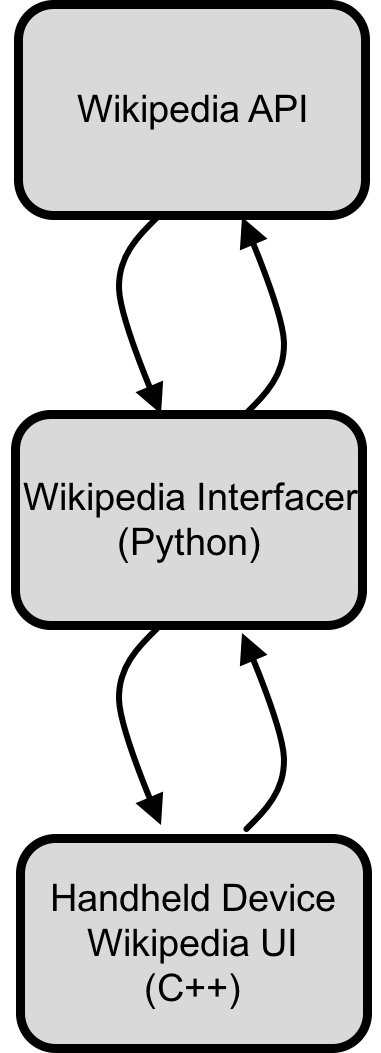
\includegraphics[scale=0.5]{wiki-block-diagram.png}
\vspace{5mm}
\caption{Block diagram for Wikipedia Scroller, from 6.S08 exercise description.}
\end{figure}


\subsection{Specification for the embedded system}
The embedded device allows its user to construct an alphanumeric query string, and it displays the results of the corresponding query.  The primary input mechanism is ``tilt", as measured by accelerometer readings.  In addition, the user can perform two actions using the push-button switch.  We define a press to be a \textit{short press} if its duration is under one second.  We define a press to be a \textit{long press} if its duration is at least one second.  The system can be viewed as an FSM with three states.  Note that, in the specifications for each state below, some of the finer details have been omitted in this paper for the sake of brevity.

\subsubsection{State 0: display state}
In this state, the result for the most recent query should be displayed.  Specifically, the screen should show as many characters as possible from the most recent HTTP (hypertext transfer protocol) response.  Initially, before any query has occurred, we define the ``most recent result" to be the empty string.  The system's built-in 5x7 fixed-size font should be used, so that eight lines, each comprised of 21 characters, can fit on the screen.  See Figure \ref{fig:pigeons} for an example.  When the user performs a long press, the system should switch to the query entry state.

\begin{figure}[t]
\centering
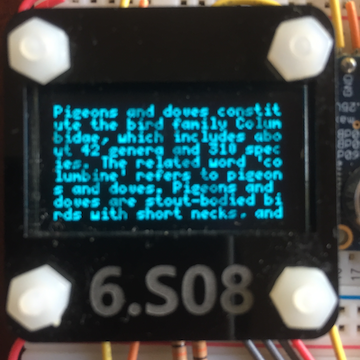
\includegraphics[width=0.5\linewidth]{text-wiki-close.png}
\vspace{5mm}
\caption{Screen output when in the display state. The last query was ``pigeons".}
\label{fig:pigeons}
\end{figure}

\subsubsection{State 1: query entry state}
In the query entry state, there are two relevant variables: \texttt{query} and \texttt{next_char_index}.  Initially, \texttt{query} is the empty string, and \texttt{next_char_index} is 0.  By definition, we say that the ``next character" is the character in the string

\begin{centering}
\texttt{"abcdefghijklmnopqrstuvwxyz0123456789"}\\
\end{centering}
\noindent at position \texttt{next_char_index}.  So, the next character is initially \texttt{"a"}.

In order to build the query string, the user selects characters one by one.  The user tilts the device left and right to ``scroll" through the possible options for the next character.  If the device is tilted $20^{\circ}$ to the right, then \texttt{next_char_index} should increment every 150 milliseconds.  If the device is tilted $20^{\circ}$ to the left, then \texttt{next_char_index} should decrement every 150 milliseconds.  The index should wrap around, so that \texttt{"9"} and \texttt{"a"} are essentially adjacent characters.

With a short press, the user ``locks in" the next character.  That is, the next character should be appended to the query string, and then \texttt{next_char_index} should be reset to 0.  Finally, with a long press, the user finishes the construction of the query string, which is then transmitted via HTTP to the server-side portion of the project.

In this state, the text on the OLED screen should always be \texttt{query}, plus the next character.  For example, if \texttt{query} is \texttt{"pigeo"} and \texttt{next_char_index} is 0, then the string \texttt{"pigeoa"} should be displayed on the screen.  Figure \ref{fig:pigeon-entry} contains six photographs taken during the process of creating a single query.

\begin{figure}
\centering
\begin{subfigure}[b]{.3\linewidth}
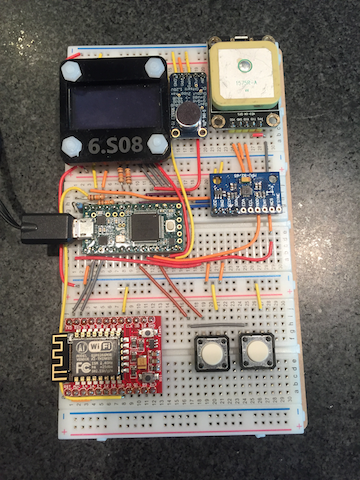
\includegraphics[width=\linewidth]{text-blank}
\caption{Screen starts blank in display mode.}
\label{fig:text-blank}
\end{subfigure}
\begin{subfigure}[b]{.3\linewidth}
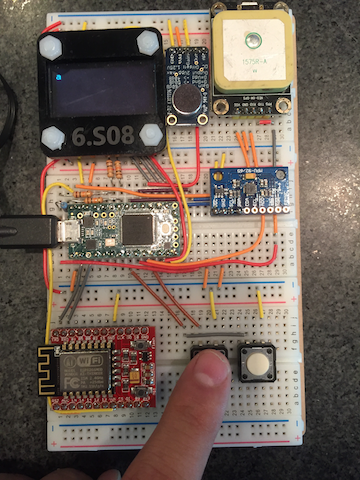
\includegraphics[width=\linewidth]{text-a}
\caption{Short press to text entry state; first letter appears.}
\label{fig:text-a}
\end{subfigure}
\begin{subfigure}[b]{.3\linewidth}
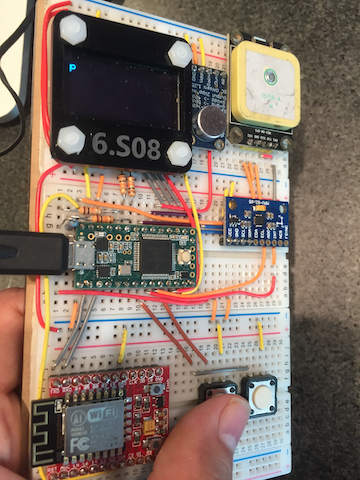
\includegraphics[width=\linewidth]{text-p}
\caption{Tilt right until first letter changes to ``p".}
\label{fig:text-p}
\end{subfigure}

\begin{subfigure}[b]{.3\linewidth}
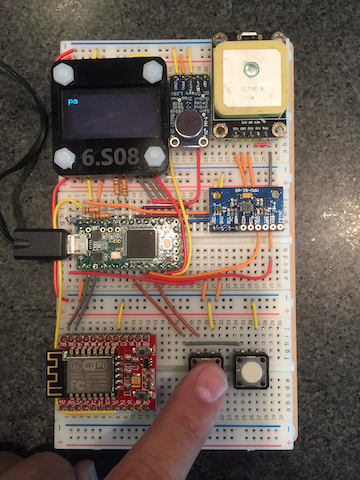
\includegraphics[width=\linewidth]{text-pa}
\caption{A short press locks in the letter; second letter appears.}
\label{fig:text-pa}
\end{subfigure}
\begin{subfigure}[b]{.3\linewidth}
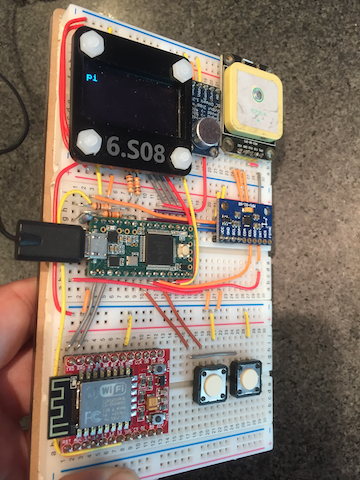
\includegraphics[width=\linewidth]{text-pi}
\caption{Tilt right until second letter changes to ``i".}
\label{fig:text-pi}
\end{subfigure}
\begin{subfigure}[b]{.3\linewidth}
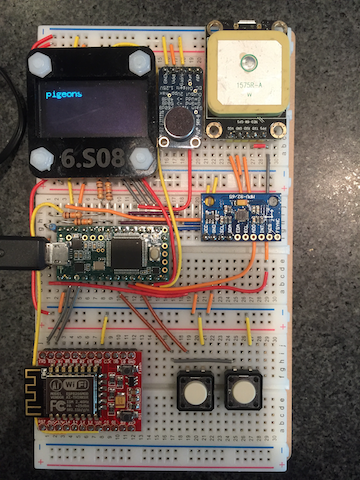
\includegraphics[width=\linewidth]{text-pigeons}
\caption{Eventually, the entire query string is entered.}
\label{fig:text-pigeons}
\end{subfigure}

\caption{Demonstration of text entry in the Wikipedia Scroller exercise.}
\label{fig:pigeon-entry}
\end{figure}

\subsubsection{State 2: waiting state}
In this state, the device waits for a response from the server.  When the response arrives, the system should transition back to the display state (which is responsible for displaying the response).  In this state, the OLED screen should contain the text \texttt{"Waiting for response"}.

\subsection{Manually grading Wikipedia Scroller}
\label{sec:manual-wiki-grade}
As a teaching assistant (TA) grading 6.S08 assignments, the author performed the following procedure to check that the assignment was implemented correctly.

First, upon system initialization, he checked that the OLED screen was blank.  Then, he performed a long press to transition to the query entry state and verified that the character \texttt{"a"} appeared on the screen.  He then tilted the device slightly left and right (less than $20^{\circ}$) to ensure the text did not change, signifying that the scroller was not too sensitive to tilt.  He would then increase the tilt to more than $20^{\circ}$ to ensure that scrolling occurred.  When holding a constant tilt at a high angle, he checked the rate at which the character changed.  He also checked that wrap-around was correctly implemented in both directions (i.e. that a left tilt from \texttt{"a"} yielded \texttt{"9"} and that a right tilt from \texttt{"9"} yielded \texttt{"a"}.

After verifying that the scrolling behavior was correct, he entered a short query string to ensure that string-building worked.  He performed a long press to send the query to the server and checked that the proper response appeared on the screen shortly thereafter.  Finally, he performed a long press to prompt a transition to query entry mode again, and verified that the old query had been cleared and the screen showed just \texttt{"a"}.

In this manner, the author was able to grade each student's work in under two minutes.  In a class of 180 students, six hours of grading time was required for this assignment alone.  Furthermore, it was difficult to give students detailed feedback, and students only received feedback after it was too late to fix any mistakes.  An automated grader would solve these problems.

\clearpage
\section{Defining a test}
In this chapter, we describe the design of the \textit{test case} data structure, and explain the reasoning behind it.  At an abstract level, MicroGrader's role is to assign a score to an embedded system.  A human grader might rely on intuition or a checklist in order to assign a score.   To automate the grading process, we must try formalize as much of this intuition as possible.  In MicroGrader, we attempt to encapsulate human intuition in the test case data structure, which defines the computation of assigning a score.  A MicroGrader test case serves two primary functions.  First, it specifies any necessary input signal signals.  Second, it specifies how the resulting output signals should be graded.

\subsection{The shortcomings of statically defined inputs}
While developing MicroGrader, we first explored a static approach to specifying inputs.  In this design, all input signals would be completely predefined.  For example, a test case could specify a digital input as seen in Figure \ref{fig:static-input}.

\begin{figure}[ht]
\centering
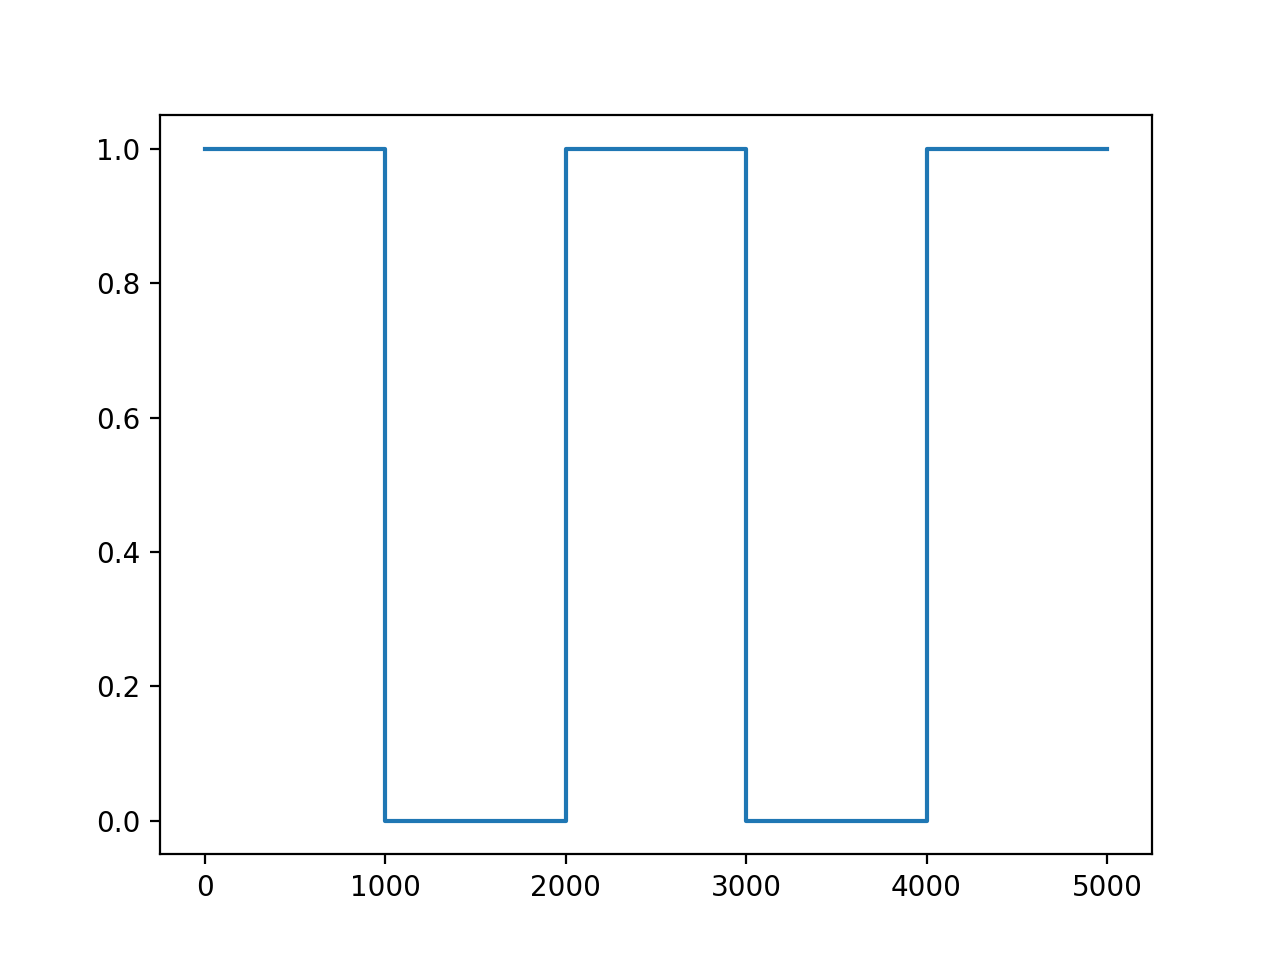
\includegraphics[scale=0.75]{button-signal.png}
\vspace{5mm}
\caption{A simple digital signal.}
\label{fig:static-input}
\end{figure}

In this particular example, presuming the digital input is connected to an active-low push-button switch, the test case indicates the button is pressed in the interval $[1000,2000)$ and $[3000,4000)$ and not pressed at all other times.  We would define $t=0$ as the time at which the microcontroller last powered on or reset.  In this static paradigm, the input signals would not depend upon the behavior of the embedded system.

In practice, we found that statically defined inputs limited the scope of assignments for which MicroGrader could be used.  Grading assignments often requires input signals that are dependent on the behavior of the system.  Consider ``Wikipedia Scroller" for a concrete example.  In particular, Wikipedia Scroller requires that the system wait for an HTTP response after transmitting a query.  The length of time spent waiting for the response varies widely and is not entirely within the student's control.  When human graders evaluate the system, they know to wait for the Wikipedia text to appear (indicating an HTTP response has arrived), before performing additional test actions.  The HTTP response might arrive less than a second after the request, or it might arrive several seconds later.  We should consider the timing of subsequent actions relative to the arrival of the HTTP response, not relative to the initialization of the system as a whole.  We can conclude that, in order to effectively grade Wikipedia Scroller, MicroGrader test cases need to dynamically define inputs, with respect to run-time events.  More generally, dynamically defined inputs allow MicroGrader to deal with variable latencies that are not within the student's control.

\subsection{Dynamically defined inputs}
We have established that MicroGrader must dynamically generate microcontroller inputs, based on the previous activity of the embedded system.  Human graders can only use system outputs to determine future input actions.  An automated grader could go further, relying on internal embedded system events in addition to system outputs.  For Wikipedia Scroller, human graders use the appearance of Wikipedia text to indicate that the HTTP response has arrived; an automated grader could, in principal, observe the arrival of the HTTP response directly and not rely on an indirect indicator.

Observing internal events directly can simplify the logic for test cases.  It is important to carefully decide which internal events MicroGrader should observe; since the grader is remotely assessing embedded system, it is impractical to observe low-level events that occur frequently.  In the current implementation of MicroGrader, the observed internal events are: ``System initialized", ``Wifi connected", ``HTTP request sent", ``HTTP response received", and ``GPS fix acquired".  In addition, MicroGrader supports a ``print" event, which allows the embedded system to send a string to the automated grader.  In general, we define a MicroGrader \textit{observation} to be one of these internal events or any external output.

\subsubsection{Data structure: ``Condition"}
\label{sec:condition}
We want the ability to specify the timing of system inputs relative to a specific, unique event that occurs during the execution of an embedded system.  In order to specify unique run-time events, we must first introduce a data structure that describes those events.  We will refer to this data structure as a \textit{condition}.  As an embedded system executes a program, MicroGrader can determine the condition's $t_{\text{satisfied}}$, the elapsed time between the embedded system's initialization and the satisfaction of the condition.  A condition's $t_{\text{satisfied}}$ can be undefined, signifying that the condition was never satisfied during the embedded system's execution.

Our condition data structure can express unique events such as: ``The first HTTP request", ``the second HTTP request", and ``the first time that the word `cat' appears on the embedded display".  It achieves this with a recursive design; complex conditions can be built by composing simpler ones.  There are four fundamental types of conditions.

The first type of condition is the \textit{BASIC condition}.  A BASIC condition's $t_{\text{satisfied}}$ is defined by a \textit{cause function}, which is boolean function that takes a single input representing a MicroGrader observation.  As MicroGrader processes each observation during the execution of an embedded program, the cause function is invoked with that observation as its input.  The condition's $t_{\text{satisfied}}$ is the \textbf{first} time at which the cause function returns \texttt{true}.  For example, we can describe ``the first HTTP request" using a BASIC condition; the cause function would return \texttt{true} if and only if the observation is an HTTP request.

The second type of condition is the \textit{AFTER condition}.  AFTER conditions have another condition (of any kind) as a ``precondition".  Like BASIC conditions, AFTER conditions have a cause function.  This cause function is only invoked for observations that occur after the precondition is satisfied.  As before, the AFTER condition's $t_{\text{satisfied}}$ is the first time at which the cause function returns \texttt{true}.  We can describe ``the second HTTP request" using this type of condition.  In particular, the precondition would be a condition signifying ``the first HTTP request", as described above.  The cause function would return \texttt{true} if any only if the observation is an HTTP request.  Note that this condition has the same cause function as the condition for ``the first HTTP request", the existence of a precondition is the only difference.  In a similar manner, we could define the \textit{n}th occurrence of any event.

Alternatively, an AFTER condition can have a cause number, $t_{\text{cause}}$, instead of a cause function.  In this case, we consider this condition's $t_{\text{satisfied}}$ to be the precondition's $t_{\text{satisfied}}$ plus $t_{\text{cause}}$.  In general, an AFTER condition cannot be satisfied without its precondition being satisfied.

The third type of condition is the \textit{AND condition}.  This type of condition has no \textit{cause}, but rather a set of subconditions, which can be of any condition type.  This condition is considered to be met once \textbf{all} of the subconditions are met.  Equivalently, this condition's $t_{\text{satisfied}}$ is the maximum of its subconditions' $t_{\text{satisfied}}$ values, or undefined if any subcondition has an undefined $t_{\text{satisfied}}$.

The fourth and final type of condition is the \textit{OR condition}.  It is analogous to the AND condition, except it is considered to be satisfied once \textbf{any} of its sub-conditions are met. Equivalently, this condition's $t_{\text{satisfied}}$ is the minimum of its subconditions' $t_{\text{satisfied}}$ values, or undefined if all subconditions have an undefined $t_{\text{satisfied}}$.  Table \ref{table:condition-summary} gives a summary of the attributes of each of the four types of conditions.

\begin{table}[ht]
\begin{center}
\begin{tabular}{cccc}
Condition Type & Cause & Precondition & Subconditions \\ \hline
BASIC & function & N/A & N/A \\
AFTER & function or number & condition & N/A \\
AND & N/A & N/A & set of conditions \\
OR & N/A & N/A & set of conditions \\ \hline
\end{tabular}
\caption{Summary of attributes of each type of condition.}
\label{table:condition-summary}
\end{center}
\end{table}

In Tables \ref{table:observations}, \ref{table:conditions}, and \ref{table:condition-descs}, we examine a concrete example showing a sequence of observations and a set of conditions, including each condition's value for $t_{\text{satisfied}}$ with respect to this set of observations.  Here, $f_{\text{httpreq}}$ and $f_{\text{high}}$ are cause functions, which take a single observation as input.  In particular, $f_{\text{httpreq}}$ returns \texttt{true} if the observation represents the sending of an HTTP request, and $f_{\text{high}}$ returns \texttt{true} if the observation represents the setting of digital output 13 to 1.  Notice that condition 4 is satisfied at $t=4000$, since both its subconditions are satisfied and the maximum of the subconditions' $t_{\text{satisfied}}$ is 4000.  By contrast, condition 5 is never satisfied because its cause function is only invoked for observations 5, 6, and 7.

\begin{table}[ht]
\begin{center}
\caption{Example observations}
\label{table:observations}
\begin{tabular}{l|lr}
& Description & Timestamp (ms) \\ \hline
Observation 1 & System initialization & 0 \\
Observation 2 & Digital output 13 set to 1 & 1000 \\
Observation 3 & HTTP request sent & 2000 \\
Observation 4 & HTTP response received & 3000 \\
Observation 5 & HTTP request sent & 4000 \\
Observation 6 & HTTP response received & 5000 \\
Observation 7 & Digital output 13 set to 0 & 6000 \\ \hline
\end{tabular}

\vspace{5mm}

\caption{Example conditions, with $t_{\text{satisfied}}$ calculated with respect to Table \ref{table:observations}}
\label{table:conditions}

\begin{tabular}{l|llllr}
& Type & Cause & Precondition & Subconditions & $t_{\text{satisfied}}$ (ms) \\ \hline
Condition 1 & BASIC & $f_{\text{httpreq}}$ & N/A & N/A & 2000 \\
Condition 2 & AFTER & $f_{\text{httpreq}}$ & Condition 1 & N/A & 4000 \\
Condition 3 & BASIC & $f_{\text{high}}$ & N/A & N/A & 1000 \\
Condition 4 & AND & N/A & N/A & Conditions 2 \& 3 & 4000 \\
Condition 5 & AFTER & $f_{\text{high}}$ & Condition 2 & N/A & Undefined \\ \hline
\end{tabular}

\vspace{5mm}

\caption{Text descriptions of example conditions from Table \ref{table:conditions}}
\label{table:condition-descs}

\begin{tabular}{l|l}
& Description \\ \hline
Condition 1 & First HTTP request sent \\
Condition 2 & Second HTTP request sent \\
Condition 3 & Digital output 13 has been set to 1 \\
Condition 4 & Digital output 13 has been set to 1 and second HTTP request sent \\
Condition 5 & Digital output 13 has been set to 1 after second HTTP request sent \\ \hline
\end{tabular}
\end{center}
\end{table}

\subsubsection{Data structure: ``Input Frame"}
Now that we have a structure for specifying run-time events, we can describe input signals relative to such events.  To do so, we introduce a new data structure called the \textit{input frame}.  An input frame consists of a start condition, an end condition, and a \textit{value generator function}.  We will refer to the start condition's $t_{\text{satisfied}}$ as $t_{\text{start}}$, and the end condition's $t_{\text{satisfied}}$ as $t_{\text{end}}$.  We say that an input frame is \textit{active} in the time interval $[t_{\text{start}}, t_{\text{end}})$.

The value generator function has two inputs: a channel, $c$, and time, $t$.  The channel, more specifically, is an input channel such as ``analog input 5" or ``accelerometer x-axis".  The value generator function returns a valid value for channel $c$ (i.e. a float for an analog channel, or $\{0,1\}$ for a digital channel).  We interpret this returned value to be the value of the input signal on channel $c$ at time $t_{\text{start}}+t$.  The value generator function should be defined for all input channels used in the exercise, and for all $t>0$.

In the context of the Wikipedia Scroller exercise, we consider an example input frame.  Suppose the frame's start condition is ``system initialization" and the end condition is ``the first HTTP request".  The two-channel value generator function, shown in Figure \ref{fig:value-gen}, specifies the input signals relative to $t_{\text{start}}$.  When a properly designed ``Wikipedia Scroller" system processes those input signals, it should: start in the display state (with a blank screen), transition to the query entry state after the long button press, scroll through a few letters due to the subsequent tilting, lock in the selected letter due to the short press, and send the one-character query string to the project's backend due to the final long press.  This process supposes a certain orientation for the IMU, which should be specified in the instructions for the exercise.

\begin{figure}[h]
\centering
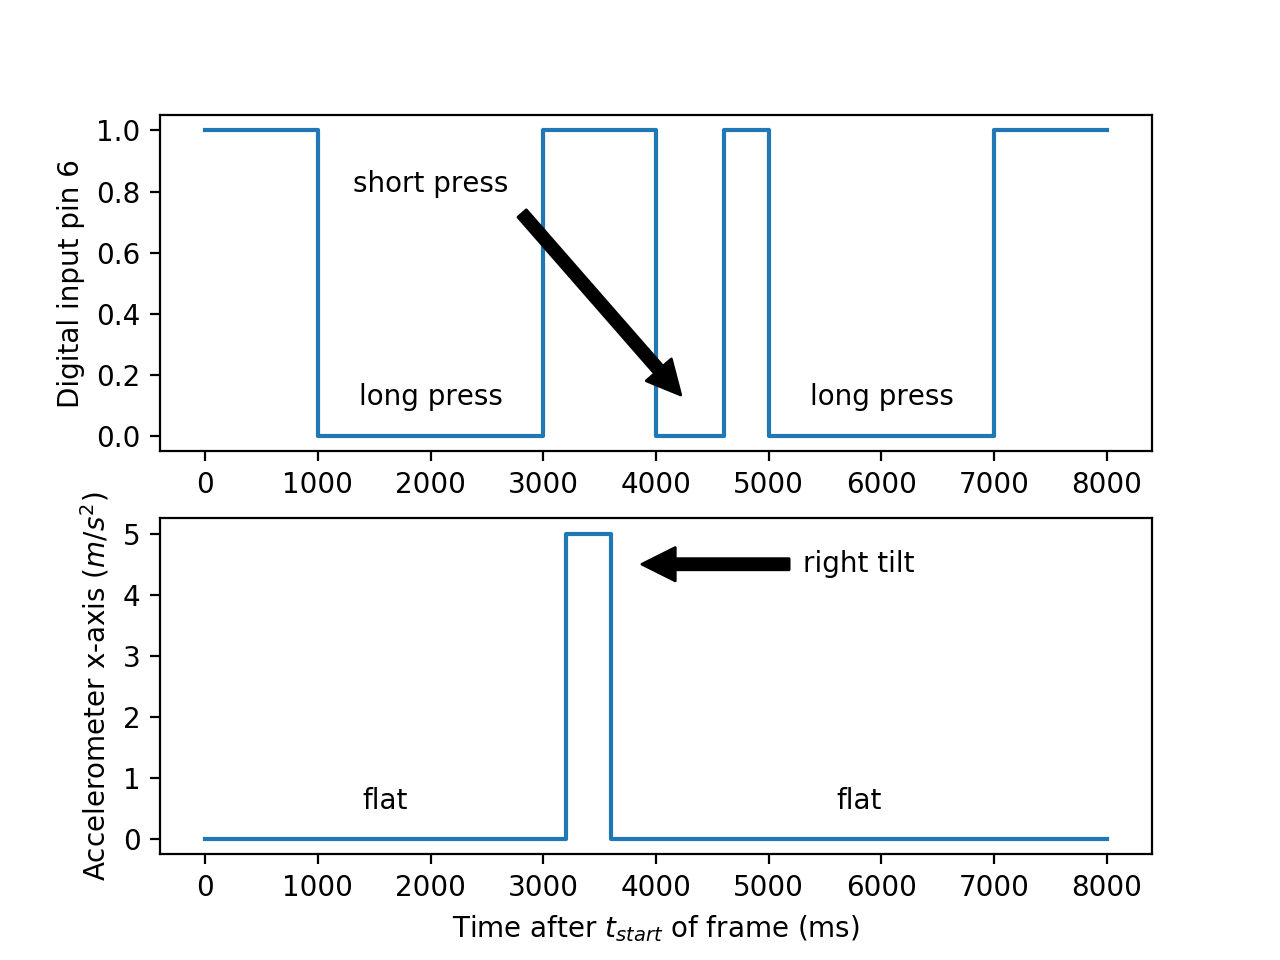
\includegraphics[scale=1]{wiki-frame.png}
\vspace{5mm}
\caption{Value generator function with two input channels.}
\label{fig:value-gen}
\end{figure}

\subsubsection{Determining input values}
A single test case usually contains multiple input frames.  At any time, MicroGrader might need to inject an input value into the embedded system.  If, at that time, a single input frame is active, we use that frame's value generator function to determine the value to inject.  We must consider the possibility that multiple input frames are active at the same time, as well as the possibility that no input frames are active.

If multiple input frames are active, we must choose which one determines the injected input value.  For this purpose, we add another attribute called \textit{priority} to our input frame data structure.  The highest priority active frame is used to determine the injected input value.  If there is a tie for the highest priority, the frame with the latest $t_{\text{start}}$ is used.  MicroGrader can be configured to instead use the frame with the earliest $t_{\text{start}}$ in a tie-breaker scenario.

If MicroGrader needs to inject an input value, and there are no active input frames, then a default value is used.  An instructor can specify a default value for any input channel.  In the case of an active-low push-button switch, it typically makes sense to use 1 as a default, indicating an unpressed button.  In the case of accelerometer readings, an instructor might want to use a default of 0 $\text{m}/\text{s}^2$ for two of the axes, and a default of 9.81 $\text{m}/\text{s}^2$ for the ``up-down" axis (due to gravity).

\subsection{Grading system outputs}
\label{sec:eval-point}
So far, we have established how MicroGrader specifies input values for a test case.  Now, we must describe how it grades the outputs of the embedded system.

MicroGrader has access to a sequence of output observations.  Output observations occur when the microcontroller generates an output.  For example, MicroGrader can observe the execution of a \texttt{digitalWrite} or \texttt{analogWrite} command on the Arduino platform, both of which specify an output voltage on a GPIO pin.  MicroGrader can also observe commands that change the embedded system's display.  Using this discrete set of output observations, MicroGrader recovers continuous output signals by assuming that outputs are constant until the next observation on the same channel.  Now, we need a method of grading a set of continuous output signals.


\subsubsection{Breaking up the grading task}
Let us consider a simple exercise, involving no inputs at all.  We will refer to this exercise as ``Blinky".  In this exercise, the microcontroller outputs a 1 Hz digital square wave on digital output 13, starting with a value of 0.  As graders, let us suppose that we only care to check the first two periods of this square wave; if these first two periods occur correctly, we will give the exercise full credit.

We define $t_{\text{start}}$ to be the time, in milliseconds, at which the embedded system finishes initializing.  Fundamentally, a grader performs four checks

\begin{itemize}
\item digital output 13 must have a value of 0 in the interval $[t_{\text{start}},t_{\text{start}}+500)$.
\item digital output 13 must have a value of 1 in the interval $[t_{\text{start}}+500,t_{\text{start}}+1000)$.
\item digital output 13 must have a value of 0 in the interval $[t_{\text{start}}+1000,t_{\text{start}}+1500)$.
\item digital output 13 must have a value of 1 in the interval $[t_{\text{start}}+1500,t_{\text{start}}+2000)$.
\end{itemize}

In the next section, we introduce a data structure called an \textit{evaluation point}, which can specify each of these four checks.

\subsubsection{Basic attributes of an evaluation point}
An evaluation point has a channel (digital output 13 in the example above) and an expected value.  It must also have an attribute that defines the time at which we expect this value.  To that end, an evaluation point has a time interval.

Since the timing of test inputs can be defined relative to run-time events, the timing of outputs can be sensitive to run-time events.  Therefore, an evaluation point also has a condition (as defined in section \ref{sec:condition}).  The evaluation point's time interval should be considered relative to the time at which the condition is met.

For ``Blinky", an instructor might consider using the four evaluation points described in Table \ref{table:blinky-basic-points} to assess a student's work.

\begin{table}[ht]
\begin{center}
\caption{A basic set of evaluation points for Blinky.}
\vspace{2mm}
\label{table:blinky-basic-points}
\begin{tabular}{c|cccc}
& Channel & Expected Value & Condition & Interval \\ \hline
Point 1 & Digital output 13 & 0 & System initialization & (0,500) \\
Point 2 & Digital output 13 & 1 & System initialization & (500,1000) \\
Point 3 & Digital output 13 & 0 & System initialization & (1000,1500) \\
Point 4 & Digital output 13 & 1 & System initialization & (1500,2000) \\ \hline
\end{tabular}
\end{center}
\end{table}

An evaluation point evaluates to either \texttt{true} or \texttt{false} with respect to a set of observed output signals.  There is no ``partial credit", since an evaluation point is our fundamental unit of grading.  If instructors want finer detail, they should create multiple separate evaluation points. 

\subsubsection{Augmenting the evaluation point for less restrictive specifications}
The evaluation points in Table \ref{table:blinky-basic-points} can verify that an embedded system implements the Blinky exercise.  In order to satisfy all four points, however, an implementation must be perfect.  That is, the rising and falling edges of the square wave must occur at exactly the correct times, to millisecond precision.  This rigidity is often undesirable in an educational context; some degree of lenience is often required in order for an academic course to avoid becoming bogged down with the finest details.

First, we augment the evaluation point data structure to allow for some timing flexibility.  Specifically, we add a new attribute called the \textit{required portion} (sometimes we will just refer to this attribute as the ``portion" for short), which is a float in the range $[0,1]$.  Using this attribute, we can relax the requirement that the student's system outputs have to be correct for the entire interval of an evaluation point.  Rather, the output value is only required to be correct for at least the specified (not necessarily contiguous) portion of the interval.  In an extreme case, a portion value of 1 implies the output must be correct for the whole interval.  At the other extreme, a portion value of $\epsilon$, a small positive value, implies the output must be correct at any time during the interval.  In our Blinky exercise, an instructor might decide to use 0.9 as the required portion, to allow for small deviations from the desired timing.

Second, we augment the evaluation point data structure to allow for value flexibility.  For certain output types, such as analog outputs, it is not appropriate to check for an exact output value.  Rather, it is usually desirable to allow for a range of allowable values.  We introduce the \textit{check function} attribute of an evaluation point to address this concern.  This function takes two inputs: the expected value and the observed value.  It returns a boolean output, indicates whether the observed value should be considered ``correct" with respect to the expected value.  For example, a check function for analog output voltages might return true if the observed value is within 0.1V of the expected value.  By default, the check function is simply the equality operator.

In Table \ref{table:blinky-lenient-points}, we can see an example of a set of points that assess the Blinky exercise with some timing flexibility.  Note that the ``channel" field has been omitted for the sake of brevity.  All of the points have ``digital output 13" as their channel.

\begin{table}[ht]
\begin{center}
\caption{A more lenient set of evaluation points for Blinky.}
\vspace{2mm}
\label{table:blinky-lenient-points}
\begin{tabular}{c|cccccc}
& Expected & Check Function & Condition & Interval & Portion \\ \hline
Point 1 & 0 & Equality operator & System initialization & (0,500) & 0.9 \\
Point 2 & 1 & Equality operator & System initialization & (500,1000) & 0.9 \\
Point 3 & 0 & Equality operator & System initialization & (1000,1500) & 0.9 \\
Point 4 & 1 & Equality operator & System initialization & (1500,2000) & 0.9 \\ \hline
\end{tabular}
\end{center}
\end{table}

Non-default check functions can be useful for evaluating screen output.  Consider our Wikipedia Scroller exercise.  An instructor might only care about the text on the screen, but not the exact positioning of the text.  In the context of this exercise, the screen is a bitmap.  The equality operator would not be an appropriate check function in this case, because it would require an exact pixel-for-pixel match between the expected bitmaps and the observed bitmaps to assess correctness.  Rather, an instructor might consider using a check function that extracts text from the bitmaps and compares the text for equality.  In fact, this particular check function is built into MicroGrader, and its implementation is detailed later in this paper.

\subsubsection{Aggregating individual point results}
\label{sec:aggregating}
For any output channel, we calculate an overall test result in a flexible way.  Specifically, an ``aggregator function" is defined for each output channel.  This function takes the set of boolean point results for that channel as input, and returns a numerical score in the interval $[0,1]$.  The scores for each output channel are then averaged together (optionally, a weighted average can be used) to get a final score for the entire test case.

\subsection{Determining the end of a test}
Embedded systems typically run indefinitely; there is no inherent ``end" to the execution of an embedded system.  Any test of an embedded system must, however, have an end.  A MicroGrader test case has an attribute called the \textit{termination condition}.  This is an instance of our usual condition data structure that, when satisfied, indicates that the test case is complete.  When constructing a test case, it is a good idea to use an end condition that is always satisfied eventually, regardless of the correctness of the student's system.  Otherwise, a test might run indefinitely, must to the student's consternation.



\clearpage
\section{Technical design }
In the introduction of this paper, we discussed that the grader and the system being graded exist in separate computing environments.  To help us describe the implementation of MicroGrader, additional terminology is helpful.  The MicroGrader \textit{server} runs on a computer, presumably a student's personal machine.  It runs the actual test case, generating inputs and collecting observations.  These observations are evaluated with respect to the test case to compute a numerical grade.

The MicroGrader \textit{client} is software running on the embedded system that allows the server to interact with the student's implementation of an exercise.  It is a thin wrapper around the input/output functionality of the embedded system.  When the student's embedded code is running, and a function is called to sample an input, the client software makes a request to the server instead of actually sampling an input from the physical sensor.  The server, in turn, responds with the test input value.  In this way, the client allows for 	``simulated" test inputs.  From the perspective of the student's code, this should be transparent; it should appear that the embedded system is receiving these inputs from sensors, even though that is not actually true.

Furthermore, the client reports observations to the server.  Whenever a student's code calls a function to generate an output, the client sends a message informing the server of this new output.  In addition, the client is responsible for reporting some internal events, such as the transmission and reception of HTTP requests.  Figure \ref{fig:test-mode} illustrates the architecture of the MicroGrader system as a whole.  All communication between the client and the server occurs via a universal serial bus (USB) connection.

\begin{figure}[h]
\centering
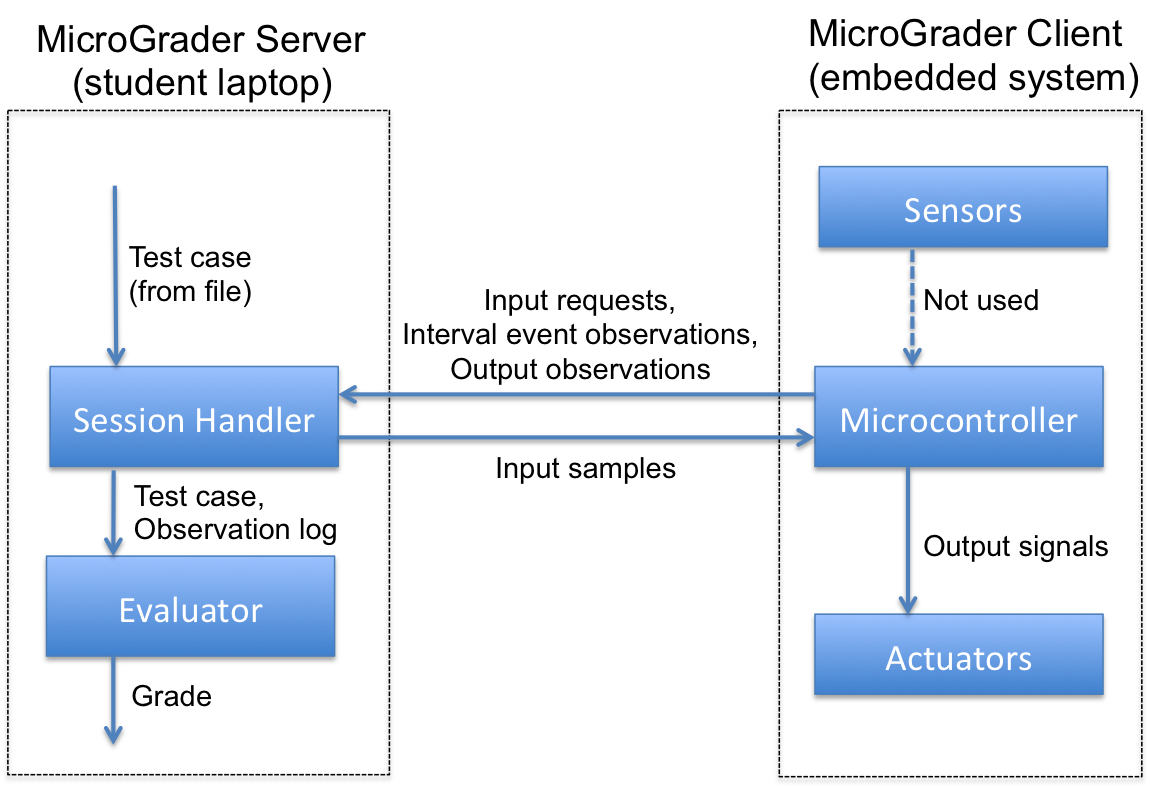
\includegraphics[width=\linewidth]{test-mode.png}
\caption{MicroGrader block diagram.}
\label{fig:test-mode}
\end{figure}

\subsection{Two-stage process}
Evaluation of a student's system occurs via a two-stage process.  First, the MicroGrader server and client engage in an interactive session to determine how the embedded system responds to test inputs.  The outputs and a narrow selection of internal microcontroller events are logged.  In the second stage, the MicroGrader server assesses the logged observations and determines an overall score for the exercise.

\subsubsection{Stage 1: The interactive session}
In this stage, the server loads the relevant test case from a file and waits for the client to connect.  Once the client connects, it begins executing the student's embedded program, sending messages to the server when appropriate.  There are, broadly speaking, two types of message from the client to the server: observations and input requests.  All messages include a timestamp, which is the number of milliseconds elapsed between the microcontroller's last reset and the time at which the message is sent.  On many microcontroller platforms, there is a built-in function for this (e.g. \texttt{millis()} on Arduino systems).  We chose to express time in milliseconds rather than microseconds, because the communication latency between the server and the client is on the order of 1 millisecond.  Sub-millisecond timing precision is therefore not very useful.

The exact contents of an observation message depend on the nature of that observation.  Output observations, for example, include the output channel and value.  Output observations are sent whenever the student's code generates an output, even if that output is redundant (i.e. the output value is identical to the previous value on the same channel).  Some observation messages contain information about internal events on the microcontroller, rather information about outputs.

When the server receives an observation message, the observation and its timestamp are logged.  In addition, for each of the test's input frames, the server examines the frame's start and end conditions, and updates them.  That is, it determines if the new observation causes these conditions to be met.  In this way, the server can keep track of which input frames are currently active, and which frame should be used to generate test inputs.  The test's termination condition is also examined, to determine if the interactive session should end.

An input request is a message from the client to the server that specifies an input channel for which a value is required.  The client sends these messages when the student's program executes a function to sample an input.  Instead of actually sampling the sensor input, the client requests a test input value.  When the server receives an input request, it determines which input frame to use to find the proper value.  It invokes the frame's value generator function, using the channel and timestamp indicated in the message.  That function returns a value, which is then sent back to the client and returned to the student's program.

\subsubsection{Stage 2: Assessment}
In this stage, the MicroGrader server considers all the activity that occurred during the interactive session.  MicroGrader scans through the activity log in order to:

\begin{itemize}
\item Determine the time at which each evaluation point's condition was met, if it was met at all.  This allows for a point's relative time interval to be converted to an absolute time interval.
\item Reconstruct all the output signals.  Recall that we assume that each the output on each channel holds until the next output on the same channel.
\end{itemize}

Each evaluation point is examined and evaluated.  Refer back to section \ref{sec:eval-point} for details.  If an point's condition was never met, then that point automatically evaluates to \texttt{false}.  The boolean results of each evaluation point are aggregated into an overall score, as per section \ref{sec:aggregating}.

MicroGrader is designed to not mask software errors.  If something goes wrong with the communication between the server and the client, or the client sends an invalid message, the session ends immediately and the test fails with an error message.  Similarly, if results of the session cannot be evaluated in the evaluation stage, the test automatically fails with an error message.  These situations are typically indicative of a malformed test case or a software bug that is not the student's responsibility.  Course staff should immediately address these types of issues.


\subsection{Implementation decisions}
\subsubsection{Client side}
When developing MicroGrader, we decided to minimize the computational responsibilities of the MicroGrader client.  We wanted to limit MicroGrader's effect on the execution of the student's embedded programs.  The students, ideally, should not notice the effect of the MicroGrader client software.  Embedded programs that meet the specification for an exercise when not connected to MicroGrader should behave similarly when MicroGrader is performing a test.

We created a implementation of the MicroGrader client for the Teensy 3.2 microcontroller development board, from PJRC \cite{teensy}, which is used as the primary computation platform for MIT's 6.S08.  It is possible, and desirable, to develop client implementations for other platforms as well.  The communication protocol, detailed in Appendix \ref{sec:teensy}, is not platform-specific.  For example, as alluded to in section \ref{sec:config}, the MicroGrader server makes no assumptions about the range and resolution of analog values.  The client is responsible for communicating range and resolution information in any analog request or observation.

We, and the original staff of 6.S08, chose to use the Teensy for a few major reasons.  Programs for the Teensy are developed using an add-on to Arduino IDE \cite{arduino-ide}.  The Arduino platform in general is popular \cite{arduino-popular}, including among students \cite{arduino-students}, and the integrated development environment (IDE) can run on Windows, MacOS, and Linux.  Many existing Arduino libraries are compatible with the Teensy, affording instructors a wide range of options for supported hardware peripherals.  The Teensy boasts impressive features for its price (under 20 dollars); it has a 72MHz 32-bit microprocessor, 34 digital input/output pins and 21 analog input pins.  It also has 64 kilobytes of random access memory (RAM) \cite{teensy-specs}.

Our client implementation for Teensy primarily consists of an embedded library that overrides certain input and output functions.  The implementations for these functions have two modes, \textit{test mode} and \textit{inactive mode}.  In test mode, the new input functions request input values from the server, rather than from sensors.  The new output functions report outputs to the server, in addition to actually sending these outputs to hardware actuators.  In inactive mode, on the other hand, input and output functions behave as if the MicroGrader library were not installed at all.  By changing the library to inactive mode, students can experiment with their solutions, without the grader interfering at all and without having to change their code significantly. 

Our Teeny client also includes slightly modified versions of existing libraries that perform input and output operations.  Similarly, our modifications enable the proper communication with the MicroGrader server.  We modified the MPU9250 library, which reads input from a digital IMU \cite{MPU9250}.  We modified the U8g2 library which can drive outputs to a variety of displays \cite{u8g2}.  Finally, we modified the 6.S08 Wifi library, so that the client can observe Wifi connectivity, HTTP requests, and HTTP responses \cite{6s08-wifi}.

Future implementations for other embedded platforms should look to the Teensy implementation as an example.  From an educational standpoint, it is valuable that the Teensy implementation requires very few changes to students' code.  The communication between the MicroGrader client and MicroGrader server is completely hidden from students.  Thanks to the inactive mode, students can work in a non-test environment without having to uninstall the test libraries.  A MicroGrader client should allow students to focus on the actual exercise at hand, not on coaxing the grader into behaving correctly.

\subsubsection{Language choice for the MicroGrader server}
We built the MicroGrader server in Python (specifically Python 3).  Python is one of the most popular programming languages \cite{python-popular}, especially in the context of education \cite{python-ed}.  Effective serial communication with embedded systems is a high priority for MicroGrader; the pyserial library is proven in the field and works on most major operating systems \cite{pyserial}. Furthermore, functions are objects in Python, which is a helpful trait since some of the attributes of our data structures are functions.  

\subsection{Reporting results}
For grading purposes, we only care about the numerical final score.  A student, however, would be well served by examining a rich and readable description of the test results.  In the event that a student does not receive full credit, this description should make it clear which points evaluated to \texttt{false} and why.

Specifically, for each evaluation point, the student can see:

\begin{itemize}
\item A text description of all the attributes of the point.
\item Whether that point evaluated to \texttt{true} or \texttt{false}.
\item A summary of the observed values on the point's channel in the point's interval.  This summary is comprised of:
\begin{itemize}
\item The unique values observed during the interval.
\item Whether or not each of those values was correct (as determined by the check function).
\item The portion of the interval for which each of those values was observed.
\end{itemize}
\end{itemize}

Some values do not lend themselves to a textual description.  For example, screen images (a very common type of output), are not easily converted to text.  To handle this, MicroGrader saves all screen images as image files in a special directory, and the text description of those images is just the file path.

For further readability, test results can be summarized somewhat more succinctly by only giving the full details for evaluation points that evaluate to \texttt{false}.  For points that evaluate to \texttt{true}, an abbreviated description can be used instead.  Students have access to both the full results and summarized results.

We considered a number of ways of reporting results to some online courseware (e.g. EdX, Coursera, etc.).  In the end, we chose a simple but effective solution, inspired by UT Austin's Embedded Systems course on EdX.  Students receive an individualized codeword for each test through the online courseware, and enter that codeword into MicroGrader.  When MicroGrader runs a test, the student's score is combined with that codeword and hashed.  The student can then copy that hash back into the courseware.  Since the number of possible scores is limited (scores are limited to four digits of precision), it's easy for the online courseware to determine the student's score.  This solution discourages cheating without requiring direct communication between MicroGrader and online courseware.  To further discourage cheating, courses could require students to upload their solutions to the online courseware for later reference.

\subsection{Screen analysis}
As previously mentioned, bitmap screens area built-in type in MicroGrader.  MicroGrader also includes some utilities for working with bitmaps, which are represented as a 2D array of binary values.  Specifically, these utilities help instructors build sensible check functions for bitmaps.  After all, exact pixel-by-pixel screen matching is often not a reasonable requirement for students.

\subsubsection{Bitmap distance metric}
MicroGrader includes a built-in distance metric for bitmaps of the same dimensions.  Specifically, we say the distance between two bitmaps is the number of pixels that do not match.  We can compute this easily by XOR-ing two bitmaps and counting the number of 1's in the result, as shown in Figure \ref{fig:naive-distance}.

\begin{figure}
\centering
\begin{subfigure}[b]{.3\linewidth}

\includegraphics[width=\linewidth]{squares-horizontal.png}
\caption{Bitmap 1, two horizontal 10x10 white squares.}
\label{fig:squares-horizontal}
\end{subfigure}
\begin{subfigure}[b]{.3\linewidth}

\includegraphics[width=\linewidth]{squares-vertical.png}
\caption{Bitmap 2, two vertical 10x10 white squares.}
\label{fig:squares-vertical}
\end{subfigure}
\begin{subfigure}[b]{.3\linewidth}
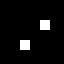
\includegraphics[width=\linewidth]{squares-diagonal.png}
\caption{XOR of bitmaps 1 and 2, showing 200 differing pixels.}
\label{fig:squares-diagonal}
\end{subfigure}
\caption{Example of using bitmap XOR to find number of pixel differences.}
\label{fig:naive-distance}
\end{figure}

This distance metric is very unforgiving of slight translations.  For example, consider two bitmaps that each represent the outline of a circle.  If one bitmap is slightly shifted relative to the other, the distance between them is quite high, as shown in Figure \ref{fig:naive-distance-problem}.  In fact, the empty (all 0s) bitmap is closer to each of these than they are to each other.  We therefore will refer to this simple distance metric as the \textit{naive distance}. A more complex distance metric seems valuable.

\begin{figure}
\centering
\begin{subfigure}[b]{.3\linewidth}

\includegraphics[width=\linewidth]{circle-left.png}
\caption{Bitmap 1, a circle at \\ location (30,30).}
\label{fig:circle-left}
\end{subfigure}
\begin{subfigure}[b]{.3\linewidth}

\includegraphics[width=\linewidth]{circle-right.png}
\caption{Bitmap 1, a circle at \\ location (35,30).}
\label{fig:circle-right}
\end{subfigure}
\begin{subfigure}[b]{.3\linewidth}

\includegraphics[width=\linewidth]{circle-diff.png}
\caption{White pixels are pixel differences.}
\label{fig:circle-diff}
\end{subfigure}
\caption{Example where two visually similar bitmaps have a large difference under the naive distance metric.}
\label{fig:naive-distance-problem}
\end{figure}


To allow for leniency with regard to translations, we introduce a parametric family of distance metrics; there are two parameters, $d_{\text{vertical}}$ and $d_{\text{horizontal}}$.  These parameters specify the maximum allowable translation of one bitmap relative to the other in the vertical and horizontal directions respectively.  The allowable vertical translations are in the range $[-d_{\text{vertical}}, d_{\text{vertical}}]$ and the allowable horizontal translations are in the range $[-d_{\text{horizontal}}, d_{\text{horizontal}}]$.  Therefore, there are a total of $(2*d_{\text{vertical}}+1)*(2*d_{\text{horizontal}}+1)$ translations in two dimensions.  To compute the distance between two bitmaps, $B_1$ and $B_2$, according to this parametrized metric, a function applies each allowable translation to $B_1$.  The distance is defined to be the minimum naive distance between $B_2$ and any of the translations of $B_1$.  For example, if we set $d_{\text{horizontal}} >= 5$, then the distance between the bitmaps in Figures \ref{fig:circle-left} and \ref{fig:circle-right} is 0.

\subsubsection{Text extraction from a bitmap}
Many assignments, such as Wikipedia Scroller, involve displaying text on a screen.  MicroGrader includes functionality to extract text from a bitmap.  At first we explored using existing tools for optical character recognition (OCR), such as tesseract \cite{tesseract}.  These generic OCR tools, however, do not perform well for small fonts.  The character glyphs of small fonts sometimes bear only vague resemblance to their counterparts in larger fonts.  For example, Figure \ref{fig:small-glyph} shows the glyph for the letter \texttt{m} in a small font from the X11 distribution \cite{5x7}.  It is difficult to develop an OCR algorithm for small fonts without prior knowledge of the exact character glyphs.


\begin{figure}
\centering

\includegraphics[width=0.3\linewidth]{glyph-m.png}
\caption{A lower-case ``m", in a 5-by-7 pixel font is difficult to recognize.}
\label{fig:small-glyph}
\end{figure}

MicroGrader's text extraction algorithm requires a bitmap representation of each character in a font.  Essentially, the algorithm scans the embedded system's output screen looking for rectangular patches that exactly match known bitmaps from a pre-loaded font.  The algorithm can be configured to ignore a subset of the characters in the font.  This is useful because some characters have glyphs that can appear in an image as a result of some other character, as shown in Figure \ref{fig:bad-ocr}.

\begin{figure}
\centering
\begin{subfigure}[b]{.3\linewidth}

\includegraphics[width=\linewidth]{glyph-T.png}
\label{fig:glyph-T}
\end{subfigure}
\begin{subfigure}[b]{.3\linewidth}
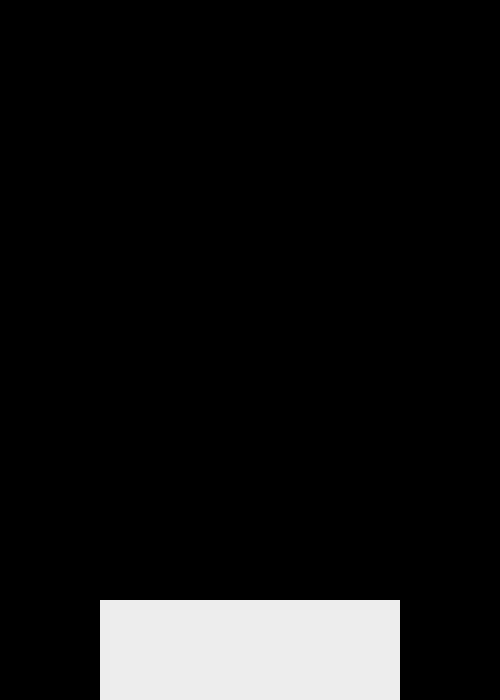
\includegraphics[width=\linewidth]{glyph-underscore.png}
\label{fig:glyph-underscore}
\end{subfigure}
\caption{The crossbar of a T is identical to an underscore character.  An instructor might choose to ignore the underscore character.}
\label{fig:bad-ocr}
\end{figure}

This text extraction algorithm is effective, but it has some weaknesses.  It requires exact glyph matches, so a single changed pixel anywhere in the rectangular window of the glyph would make the character unrecognizable to the algorithm.  The algorithm requires each glyph in the font before performing any recognition; instructors must provide the font data.

\subsection{Configurability and defaults}
\label{sec:config}
MicroGrader is designed to be as configurable as possible.  This manifests itself in a variety of ways.  Test cases themselves are highly configurable, as described earlier.  Furthermore, certain design decisions were made in order to make MicroGrader compatible with as many embedded platforms as possible.  For example, it makes no assumptions about the resolution at which to discretize analog values.  Any request for an analog input or observation of an analog output comes packaged with information about the desired range and resolution of the analog quantity.

Later, it will be possible to add additional data types, beyond the built-in ones, without changing the source code.  The easiest way to do this is by importing serialized \cite{pickle} Python objects that include implementations of all the functions a data type needs to have.  The minimum functions for a new data type are: serialization, deserialization, and a definition of the equivalence operator.

The high level of configurability could potentially make it difficult for an instructor to use MicroGrader.  Therefore, wherever possible, reasonable defaults are included.  For example, consider the aggregator function, which maps a list of evaluation point results to a score.  By default, each channel uses a ``proportional" aggregator function, where the score is just the fraction of points that evaluate to \texttt{true}.  An instructor could replace this with any valid aggregator, such as an ``all-or-nothing" function which returns 1 if all points evaluate to \texttt{true} and 0 otherwise.


\clearpage
\section{Limitations}
Although MicroGrader is well-suited for grading many types of microcontroller projects, there are limitations that any instructor using this tool should know about.  Awareness of these limitations would help instructors design technical specifications that MicroGrader can assess effectively.

\subsection{Latency}
In order to implement its side of the protocol, embedded clients must do some computational work.  Effort has been made to minimize this, but nevertheless MicroGrader is unsuitable for projects that have very sensitive timing, or that involve performing I/O operations at high frequencies.  For example, the latency of sampling an input is often order of magnitude (or two) higher when the MicroGrader client is in use, compared to regular microcontroller operation.  The embedded client must wait for the MicroGrader server to process and respond to a request for an input value.  Most of the latency is fundamentally due to the round-trip latency of the USB protocol.

The latency issue makes is impossible for MicroGrader to observe device-level communication channels such as UART (universal asynchronous receiver/transmitter), $\text{I}^2\text{C}$ (inter-integrated circuit), or SPI (serial peripheral interface), or to inject values into those channels at a reasonable rate.  If the MicroGrader client tried to report each $\text{I}^2\text{C}$ message to the server, for example, the data throughput on the $\text{I}^2\text{C}$ would drop precipitously.

The specific constraints depend on the platform.  In building the reference implementation for Teensy, I observed that round-trip latency for relatively small messages ($<100$ bytes) was about a millisecond.  Therefore, the upper bound for the input sampling rate is around 1 KHz.  This is fast enough for many assignments that involve ``human" time scales, but insufficient in other cases, such as audio sampling.

\subsection{Point-by-point evaluation}
Our evaluation point structure inherently forces a test case to independently evaluate points of an output signal.  For any given interval, there is a single expected value.   A more sophisticated correctness metric, involving the entire output signal at once, aren't possible in this framework.  For example, we cannot use evaluation points to determine the cross-correlation between the observed output signal and an expected output signal.

\subsection{Sensitivity to time scaling}
Evaluation points have time intervals that are fixed, relative to the satisfaction of a condition.  If a student's solution shifts its outputs time-wise, it could cause many of the points to evaluate to \texttt{false}.  The overall output signals might appear reasonable, while being ``out-of-phase" with the expected signal, so to speak.  As a concrete example, consider a student implementation of Wikipedia Scroller where the ``scrolling" in text entry mode occurred 10\% too slowly.  That is, the letters change every 165 milliseconds instead of every 150 milliseconds.  To a human grader, this difference would probably be imperceptible.  In fact, an instructor might want to give some lenience for issues like this.  The system's outputs would be delayed relative to the expected solution, and there is currently no easy way to configure MicroGrader to handle that leniently.

\subsection{Step-wise constant restriction}
MicroGrader assumes that the embedded system's outputs remain constant until the next output is observed.  While a step-wise constant function can approximate any step-wise continuous function to arbitrary precision, this can put an unacceptably high burden on the embedded client.  For example, both the Teensy has built-in functionality for creating square wave signals of a specified frequency for a specified duration, using a single user-facing instruction (\texttt{tone(pin, frequency)} or \texttt{tone(pin, frequency, duration)}).  In order for the embedded client to properly inform the server about the square wave signal, it would have to send a message on every rising and falling edge.  It is not possible, in a single message, to inform the server about the square wave that is being produced.

\subsection{Derived outputs}
\label{sec:derived-outputs}
In many systems, the embedded device produces outputs that serve as inputs to some physical plant, which then produces the outputs we actually care about.  For example, a microcontroller might drive the voltage across the terminals of a motor, connected to a wheel.  Perhaps we care only about the position of the wheel, not the motor's terminal voltage.  Even under the assumption that the motor's angular velocity is proportional to the terminal voltage, and the motor responds instantaneously, we would have to integrate the microcontroller's output to derive the pertinent physical output.

It is currently impossible to evaluate derived outputs like this using MicroGrader (unless the derived output is zeroth order linear function of the microcontroller's output).  In a later version, MicroGrader will include the ability to add a custom physical model to convert the raw output into a derived output.

\clearpage
\section{Automatic test generation}
So far in this paper, we have described a structure for defining tests and a technical system capable of carrying out those tests.  Creating a test case, however, can be a tedious process.  Instructors must define each input frame, including the value generator function for each input frame.  Value generator functions, which define a value for every input channel at every time $t>0$ can be complicated.  In Figure \ref{fig:value-gen} from section \ref{sec:wiki-scroller}, we showed how a value generator function could define inputs.  In the context of Wikipedia Scroller, these particular input signals would yield a query string of length 1.  Creating a longer query string, and triggering the edge cases described in section \ref{sec:manual-wiki-grade}, would require significantly more complex inputs and implementing the value generator function would become time-consuming.

Specifying evaluation points for assessing an implementation of Wikipedia Scroller can also be tedious.  A human grader, while performing the manual grading process for the exercise, observed dozens of unique screen outputs.  For each output that the instructor deems relevant, the MicroGrader test would have to have an evaluation point.  The instructor would be responsible for determining the timing and expected value (a 128x64 bitmap) for each of these points.

The primary purpose of MicroGrader is to streamline the grading process, so it is important to make it easy and intuitive to create test cases.  To this end, we have built a utility for MicroGrader that allows an instructor to automatically generate a test case using a reference solution for the exercise.

\subsection{Recording a reference solution}
In order to obtain a recording of a correctly implemented solution, we use introduce a mode of operation called \textit{recording mode}.  Recording mode differs from regular testing in that input values are \textbf{not} predefined.  Rather, inputs are sampled by the embedded system's sensors and those values are reported to the MicroGrader server, as shown in Figure \ref{fig:recording-mode}.

\begin{figure}[ht]
\centering
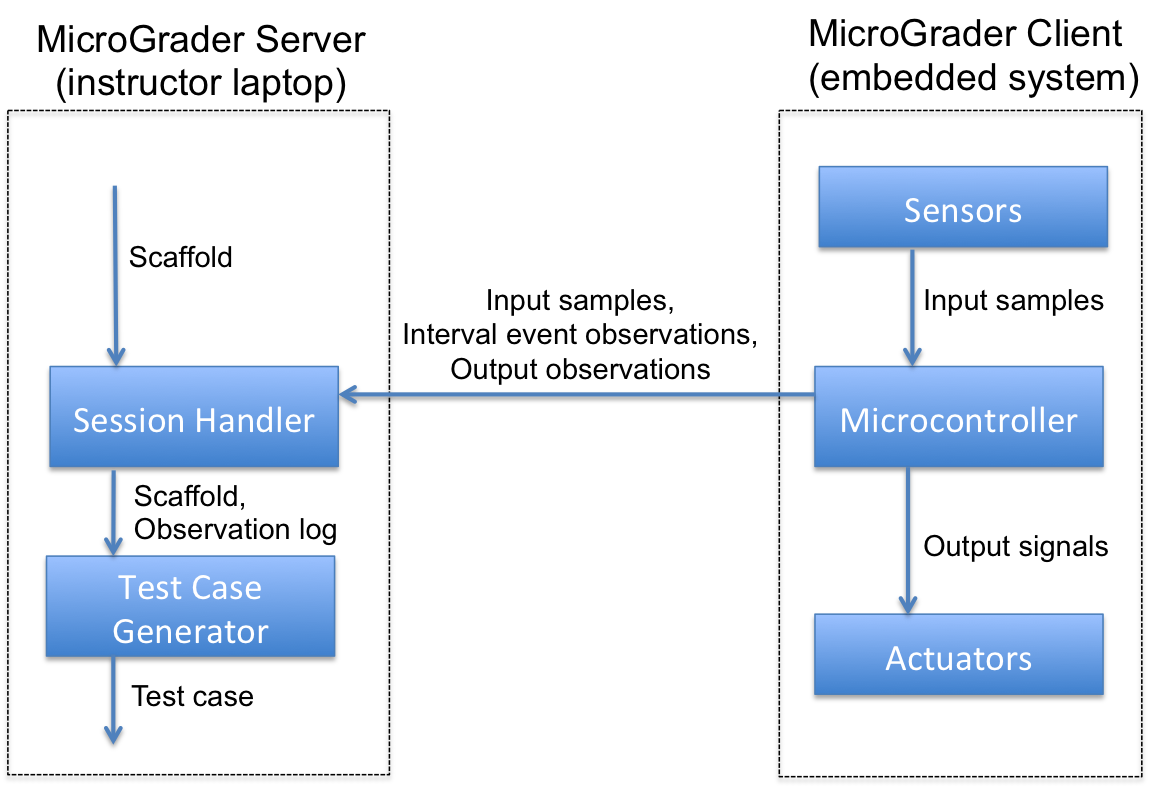
\includegraphics[width=\linewidth]{recording-mode.png}
\caption{MicroGrader block diagram in recording mode.}
\label{fig:recording-mode}
\end{figure}

An instructor with a working solution can use this mode to perform some set of tasks that fully demonstrate the functionality of the system.  Meanwhile, the MicroGrader server compiles a full record of observations of the embedded system's, including input values.  Those observations are then used to programmatically construct a test case.

It is difficult to define a test case using observations alone.  There are many ambiguities in terms of how an instructor might want to the assignment to be graded.  MicroGrader test cases define inputs dynamically, relative to a condition; a test generator would have to determine the conditions relative to which input signals should be defined.  Furthermore, an instructor might only want to assess system outputs during certain periods of time, and ignore other periods.  For example, a Wikipedia Scroller test might be set up in such a way that ignores system outputs when the embedded system is waiting for an HTTP response.

The evaluation point data structure allows instructors to specify check functions, which afford leniency to output values that are not exactly correct.  Evaluation points also allow instructors to specify a time interval and a ``required portion" of that interval for which the output should be correct.  A test generator would have to account for instructors' preferences with regards to these attributes.

MicroGrader uses a data structure called the \textit{scaffold} to allow for instructors to specify these preferences.  The scaffold and the observations of a reference solution, when combined, can be used to produce a full test case.

\subsection{Frame templates}
First, we will focus on automatically constructing the input frames of a test.  After exploring a few methods of doing this, we decided that instructors should specify the start and end conditions of each frame in the generated test; perhaps we should refer to our test construction procedure as ``semi-automatic".  Typically, the tedious aspect of building input frames is specifying the value generating function, while specifying the start and end conditions is relatively easy.

Our manual grading process for Wikipedia Scroller involved a complicated query entry process, then sending a query to the project's backend, then displaying the response from the back-end, and finally restarting the query entry process.  In this case, a scaffold for automatically building a test might have two input frames, as shown in Table \ref{table:frame-templates}.

\begin{table}[ht]
\begin{center}
\vspace{2mm}
\begin{tabular}{c|ll}
& Start condition & End condition \\ \hline
Frame 1 & System initialization & $1^{\text{st}}$ HTTP request sent \\
Frame 2 & $1^{\text{st}}$ HTTP response received & 6 seconds after first HTTP response received \\ \hline
\end{tabular}
\caption{A more lenient set of evaluation points for Blinky.}
\label{table:frame-templates}
\end{center}
\end{table}

Frame 1 would specify the inputs required to begin the first query entry process, perform out that entry process, and send the query.  Frame 2 would specify the inputs required to restart the query entry process after the HTTP response arrives.  An instructor specifies the start and end conditions; it is the role of our test construction algorithm to add the value generating functions.

\subsection{Building value generating functions}
The first step in constructing our value generating functions is to convert the observed discrete input signals to continuous input signals.  Suppose that on some input channel, the \textit{n}th sample occurs at time $t_n$, the previous sample occurs at time $t_{n-1}$, and the subsequent sample occurs at time $t_{n+1}$.  MicroGrader offers several ways to create a continuous signal using these samples:

\begin{itemize}
\item Post-hold: the \textit{n}th sample is valid in the interval $[t_n, t_{n+1})$.
\item Pre-hold: the \textit{n}th sample is valid in the interval $(t_{n-1}, t_n]$.
\item Mid-hold: the \textit{n}th sample is valid in the interval $[(t_{n-1} + t_n)/2, (t_n + t_{n+1})/2)$.
\item Interpolation: Values between samples are determined using linear interpolation. 
\end{itemize}

These methods are illustrated in Figure \ref{fig:interpolation}.  Instructors can specify a different method of creating the continuous signal for each input channel.  For some types of input channels, namely digital ones, the ``interpolate" method is not valid.

\begin{figure}
\centering
\begin{subfigure}[b]{.45\linewidth}
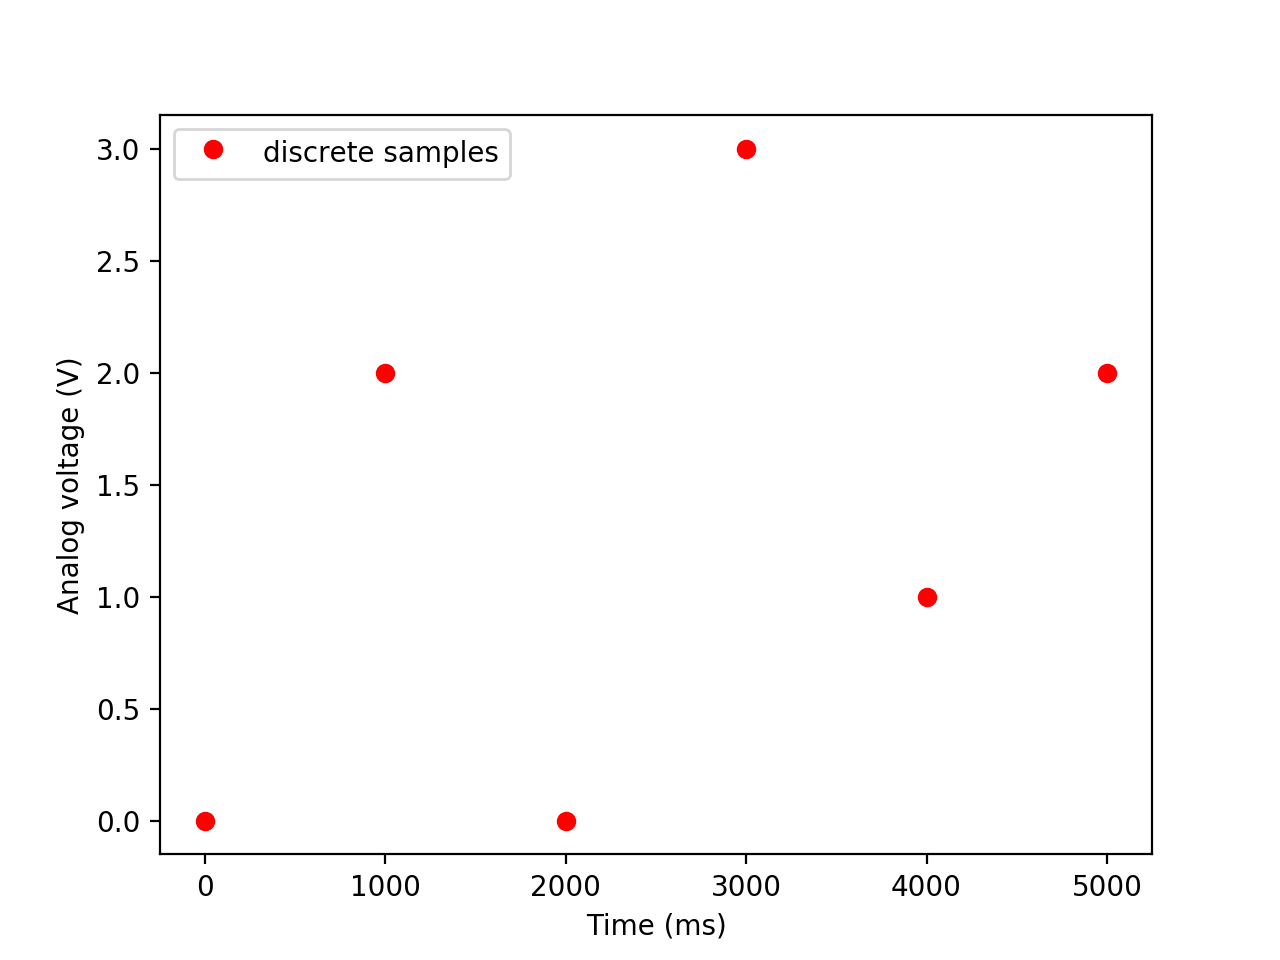
\includegraphics[width=\linewidth]{input-samples.png}
\caption{Input samples.}
\end{subfigure}

\begin{subfigure}[b]{.45\linewidth}
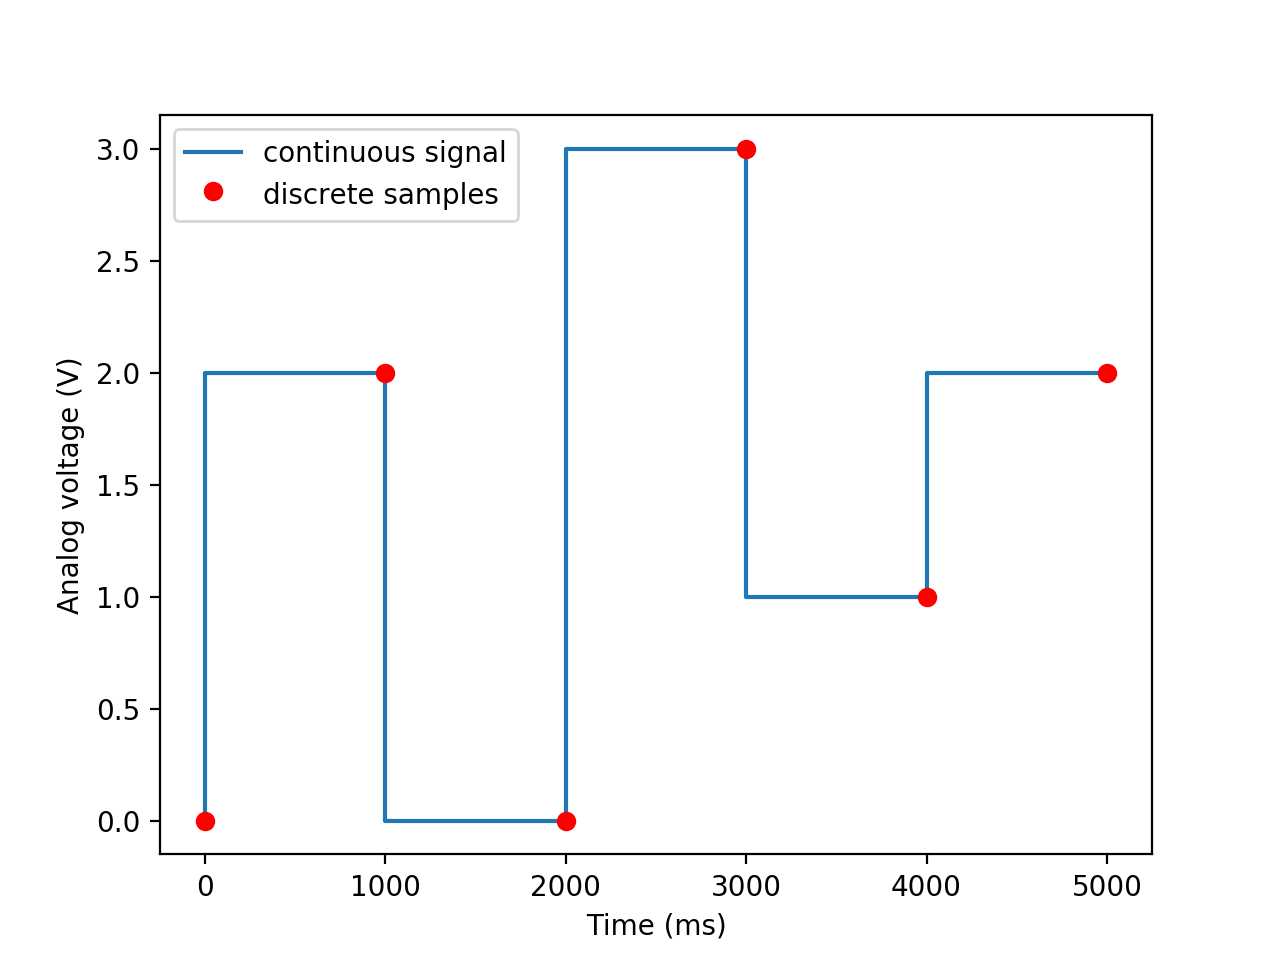
\includegraphics[width=\linewidth]{input-pre.png}
\caption{Pre-hold continuous signal.}
\end{subfigure}
\begin{subfigure}[b]{.45\linewidth}
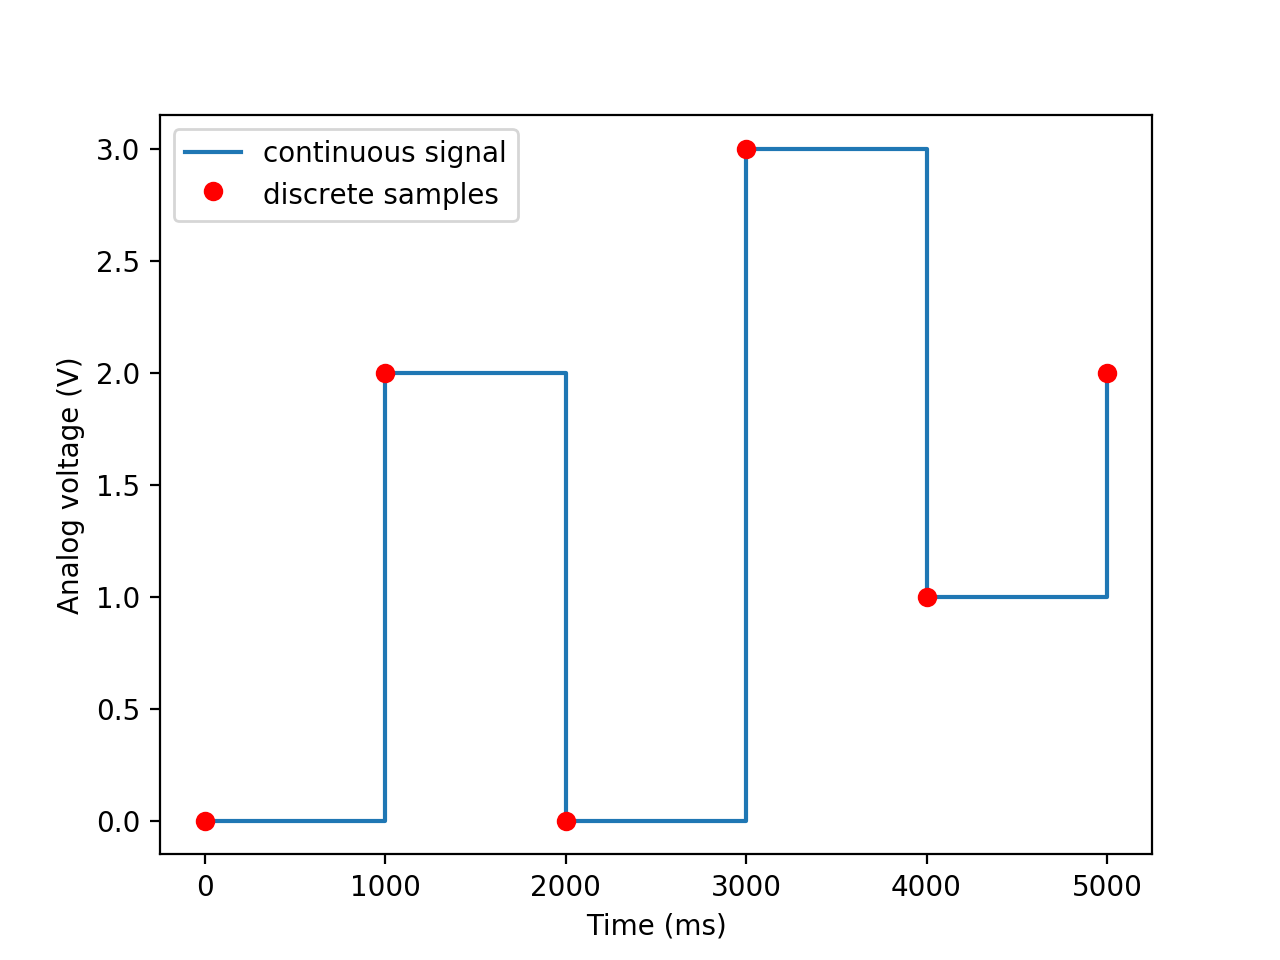
\includegraphics[width=\linewidth]{input-post.png}
\caption{Post-hold continuous signal.}
\end{subfigure}

\begin{subfigure}[b]{.45\linewidth}
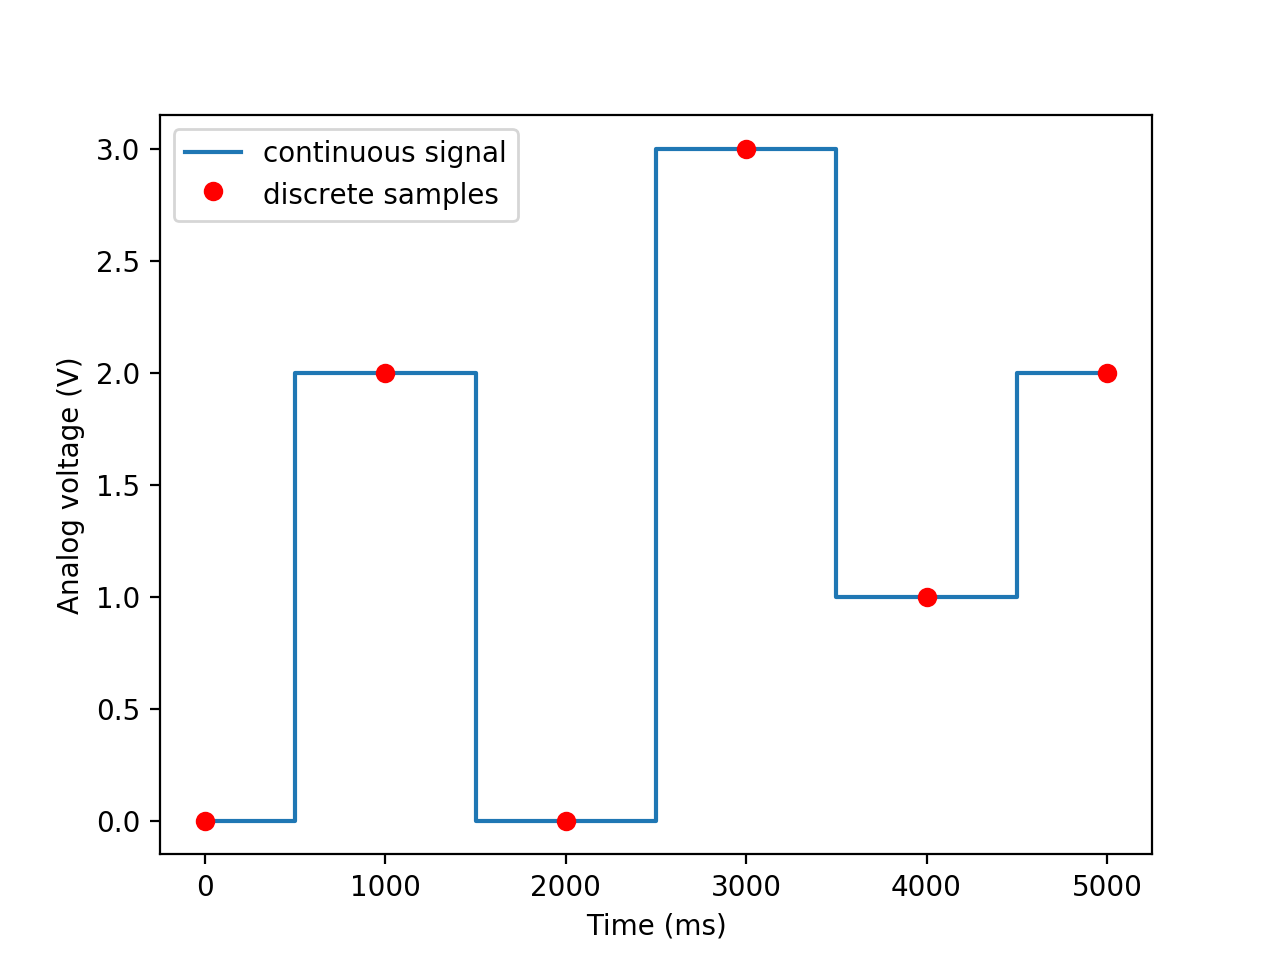
\includegraphics[width=\linewidth]{input-mid.png}
\caption{Mid-hold continuous signal.}
\end{subfigure}
\begin{subfigure}[b]{.45\linewidth}
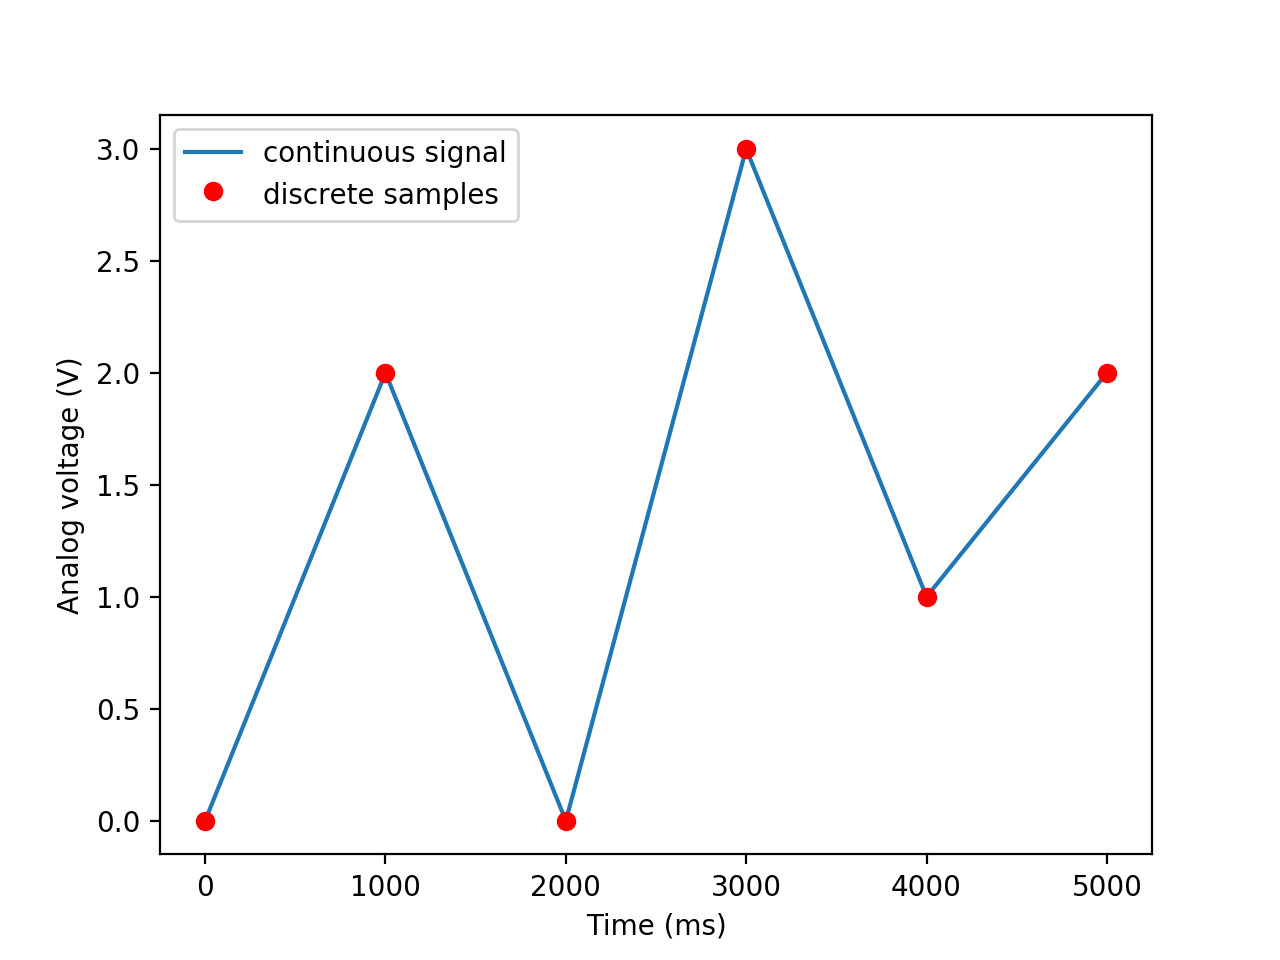
\includegraphics[width=\linewidth]{input-inter.png}
\caption{Interpolated continuous signal.}
\end{subfigure}
\caption{Examples of Micrograder's four built-in methods of generalizing a discrete signal.}
\label{fig:interpolation}
\end{figure}

After converting the discrete input signals to continuous input signals, our algorithm uses these signals to determine the value generating function for each input frame.  First, it examines the observation log to determine the $t_{\text{start}}$ and $t_{\text{end}}$ for each input frame in the scaffold.  Recall that $t_{\text{start}}$ and $t_{\text{end}}$ are the $t_{\text{satisfied}}$ times for the start and end conditions, respectively, of an input frame.  For any input frame, if either of $t_{\text{start}}$ or $t_{\text{end}}$ are undefined, or $t_{\text{start}}$ >= $t_{\text{end}}$, then that input  frame is discarded and will not be included in our constructed test.

For each remaining input frame, we can now determine the value generating function.  Specifically, for each input channel, we extract the portion of the signal between $t_{\text{start}}$ and $t_{\text{end}}$ of the frame.  We translate this signal so that it begins at $t=0$, and we extend the signal from its final value (which was originally at $t=t_{\text{end}}$) to infinity.  This process is illustrated in Figure \ref{fig:input-framing}.

\begin{figure}[ht]
\centering
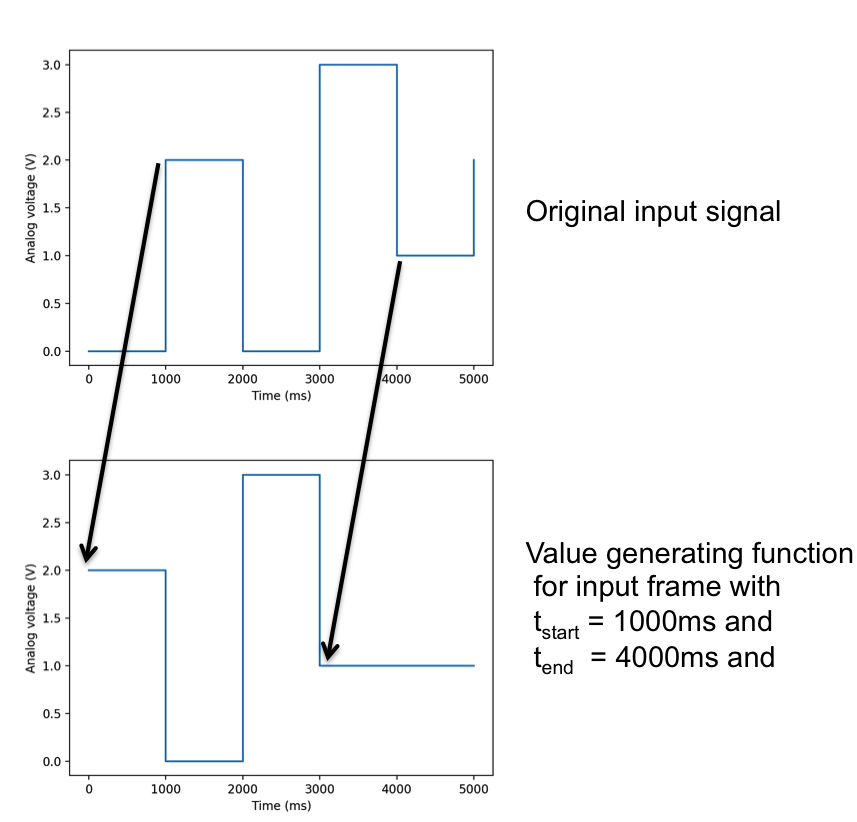
\includegraphics[width=0.6\linewidth]{input-framing.png}
\caption{Visualization of building a value generating function for a single analog input channel.}
\label{fig:input-framing}
\end{figure}

\subsection{Constructing evaluation points}
\label{sec:using-point-templates}
As with constructing input frames, the first step is converting discrete output observations to continuous signals.  In this case, we use the ``post-hold" method described in the previous section.  Also from the previous section, we have the $t_{\text{start}}$ and $t_{\text{end}}$ times for each frame.  For each frame, we consider the interval $[t_{\text{start}}, t_{\text{end}})$ of each output signal, and translate it so that it begins at $t=0$.  So far, this is the same process as we performed with input signals, except we do not extrapolate the output signal to $t=\infty$, as shown in Figure \ref{fig:output-framing}.  We will refer to this piece of the original output signal as the \textit{reference signal}.  

\begin{figure}[ht]
\centering
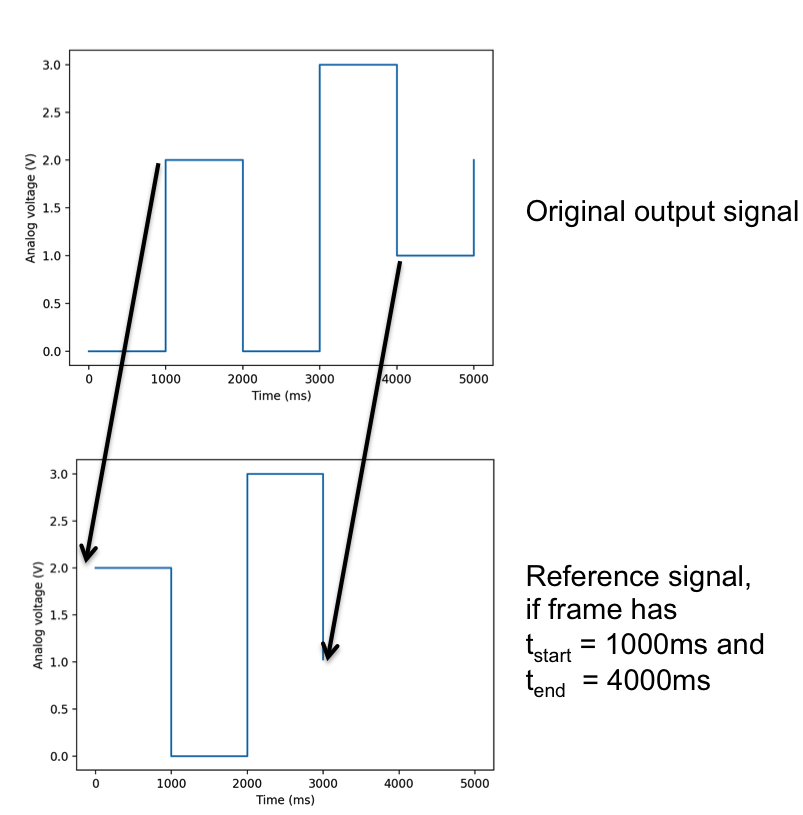
\includegraphics[width=0.6\linewidth]{output-framing.png}
\caption{Visualization of extracting a portion of an output signal.}
\label{fig:output-framing}
\end{figure}

Recall that since this is a recording of an instructor's embedded system, its outputs are correct by definition.  Now, our task is to generate a set of evaluation points that can represent this interval of the expected output signal.  For the sake of clarity, we will continue to focus on a reference signal for a single output channel within a single frame, but the process of creating and using a reference signal is the same for all frames and output channels.  We'll refer to the start condition of our hypothetical frame as $C_{\text{start}}$.

First, we partition the reference signal into intervals with constant value.  In this case, there are three such intervals: $(0,1000)$,$(1000,2000)$, and $(2000,3000)$.  For each of these constant-value intervals, we construct one evaluation point that determines whether another signal matches the reference signal in this interval, as shown in Table \ref{table:construct-points}.

\begin{table}[ht]
\begin{center}
\caption{Evaluation points to assess reference signal from Figure \ref{fig:output-framing}.}
\vspace{2mm}
\label{table:construct-points}
\begin{tabular}{cccccc}
Expected Value & Check Function & Condition & Interval & Portion \\ \hline
2.0 V & ? & $C_{\text{start}}$ & (0,1000) & ? \\
0.0 V & ? & $C_{\text{start}}$ & (1000,2000) & ? \\
3.0 V & ? & $C_{\text{start}}$ & (2000,3000) & ? \\ \hline
\end{tabular}
\end{center}
\end{table}

The start and end time of each constant-value interval define the ``time interval" attribute of the corresponding evaluation point.  Recall that we defined $t=0$ in our reference signal to be the time at which $C_{\text{start}}$ was satisfied, so $C_{\text{start}}$ is the condition for each evaluation point.  The expected value for each evaluation point is the value of the reference signal in the corresponding interval.

As observed in the table, we have no way to determine the proper check function for the evaluation points.  Similarly, we cannot determine the ``portion" attribute, which essentially tunes the leniency of the evaluation point.  These two attributes are used to make evaluation points more flexible, and are inherently not specified by the reference signal, but rather by instructors.  Therefore, our scaffold data structure includes instructors' preferences for these attributes.  Instructors can specify a check function and portion for each output channel.  Table \ref{table:construct-points-2} shows some reasonable choices.

\begin{table}[ht]
\begin{center}
\caption{Evaluation points to assess reference signal from Figure \ref{fig:output-framing}.}
\vspace{2mm}
\label{table:construct-points-2}
\begin{tabular}{cccccc}
Expected Value & Check Function & Condition & Interval & Portion \\ \hline
2.0 V & True if values are within 0.1 V & $C_{\text{start}}$ & (0,1000) & 0.8 \\
0.0 V & True if values are within 0.1 V & $C_{\text{start}}$ & (1000,2000) & 0.8 \\
3.0 V & True if values are within 0.1 V & $C_{\text{start}}$ & (2000,3000) & 0.8 \\ \hline
\end{tabular}
\end{center}
\end{table}

The last part of a test is the aggregator function, which defines how a set of boolean evaluation point results are combined into a numerical grade.  As with the check function and portion attributes, the aggregator function is specified by instructors on a per-channel basis.  A typical aggregator function is the function that returns the fraction of points that evaluate to \texttt{true}.

\subsection{Auto-generated test case for Wikipedia Scroller}
To demonstrate the capability of the test construction algorithm, we used it to build a test for Wikipedia Scroller.  For our scaffold, we started with the frames from Table \ref{table:frame-templates}, shown again in Table \ref{table:frame-templates-2} for convenience.

\begin{table}[ht]
\begin{center}
\vspace{2mm}
\begin{tabular}{c|ll}
& Start condition & End condition \\ \hline
Frame 1 & System initialization & $1^{\text{st}}$ HTTP request sent \\
Frame 2 & $1^{\text{st}}$ HTTP response received & 6 seconds after first HTTP response received \\ \hline
\end{tabular}
\caption{A more lenient set of evaluation points for Blinky.}
\label{table:frame-templates-2}
\end{center}
\end{table}

For the recording, we performed a minimal test procedure that mostly covers the intended functionality of the system.  After initialization, we entered the query-entry state with a long press, scrolled left to the ``9" character, scrolled right to the ``c" character, locked that character in with a short press, and then sent the query with a long press.  After the response arrived, we entered the query-entry state with a long press again, and locked in the letter ``a" with a short press.

In the recording, two input samples were taken on two channels: a digital input connected to the active-low push-button switch, and the x-axis of an accelerometer which gives us information about the left-right tilt of the embedded system.  Based on the recording, MicroGrader created value generating functions for each of the two frames, as illustrated in Figure \ref{fig:actual-input-frames}.  At a glance, one can see the actions that occurred during the recording. Frame 1 consists of a long press, followed by some tilting, following by a short press, and finally a long press.  Frame 2 consists of a long press followed by a short press, with very little tilting.

\begin{figure}[ht]
\centering

\begin{subfigure}[b]{.45\linewidth}
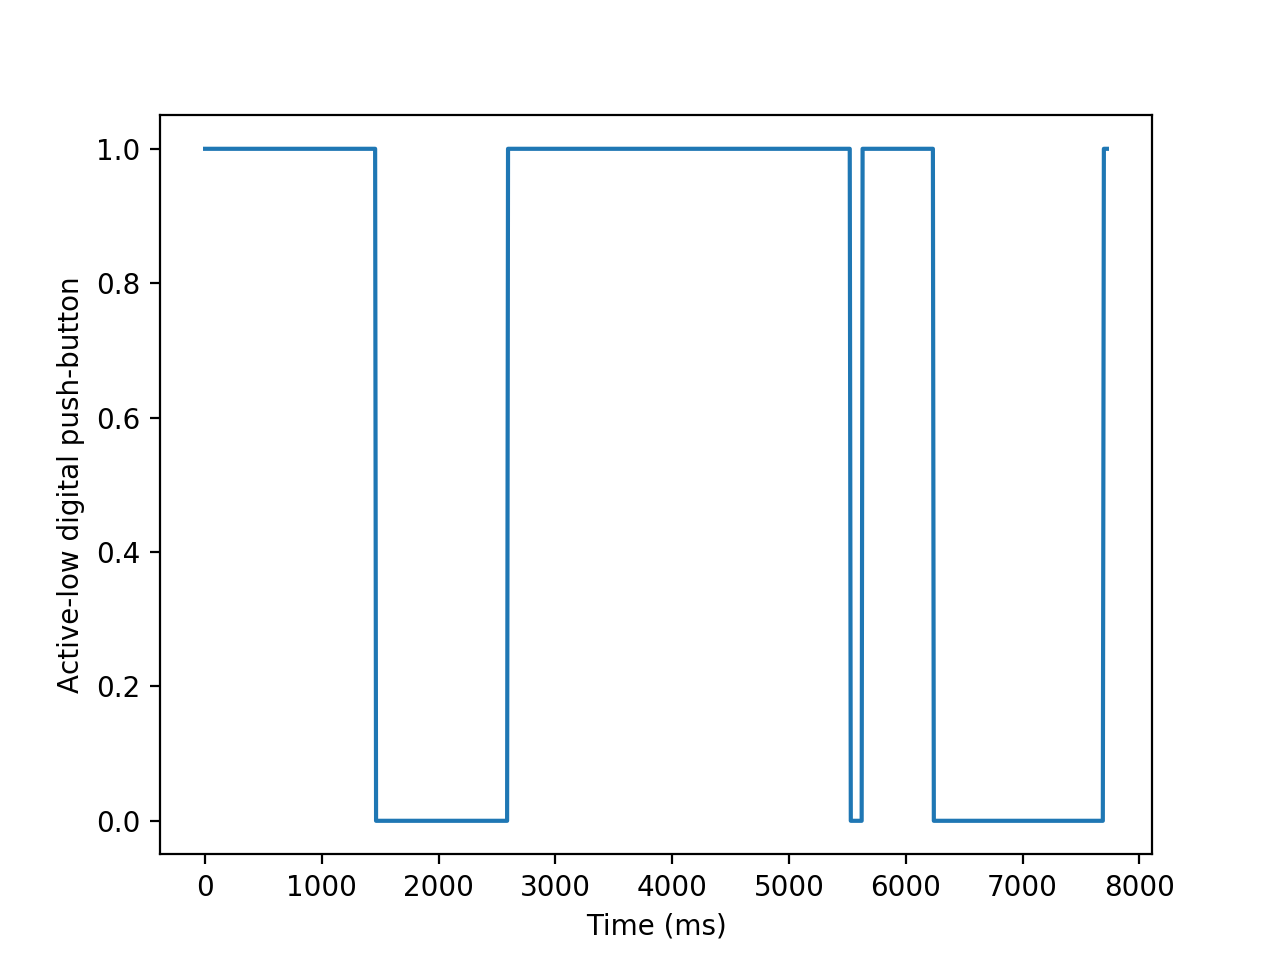
\includegraphics[width=\linewidth]{f0-button.png}
\caption{Frame 1, button input.}
\end{subfigure}
\begin{subfigure}[b]{.45\linewidth}
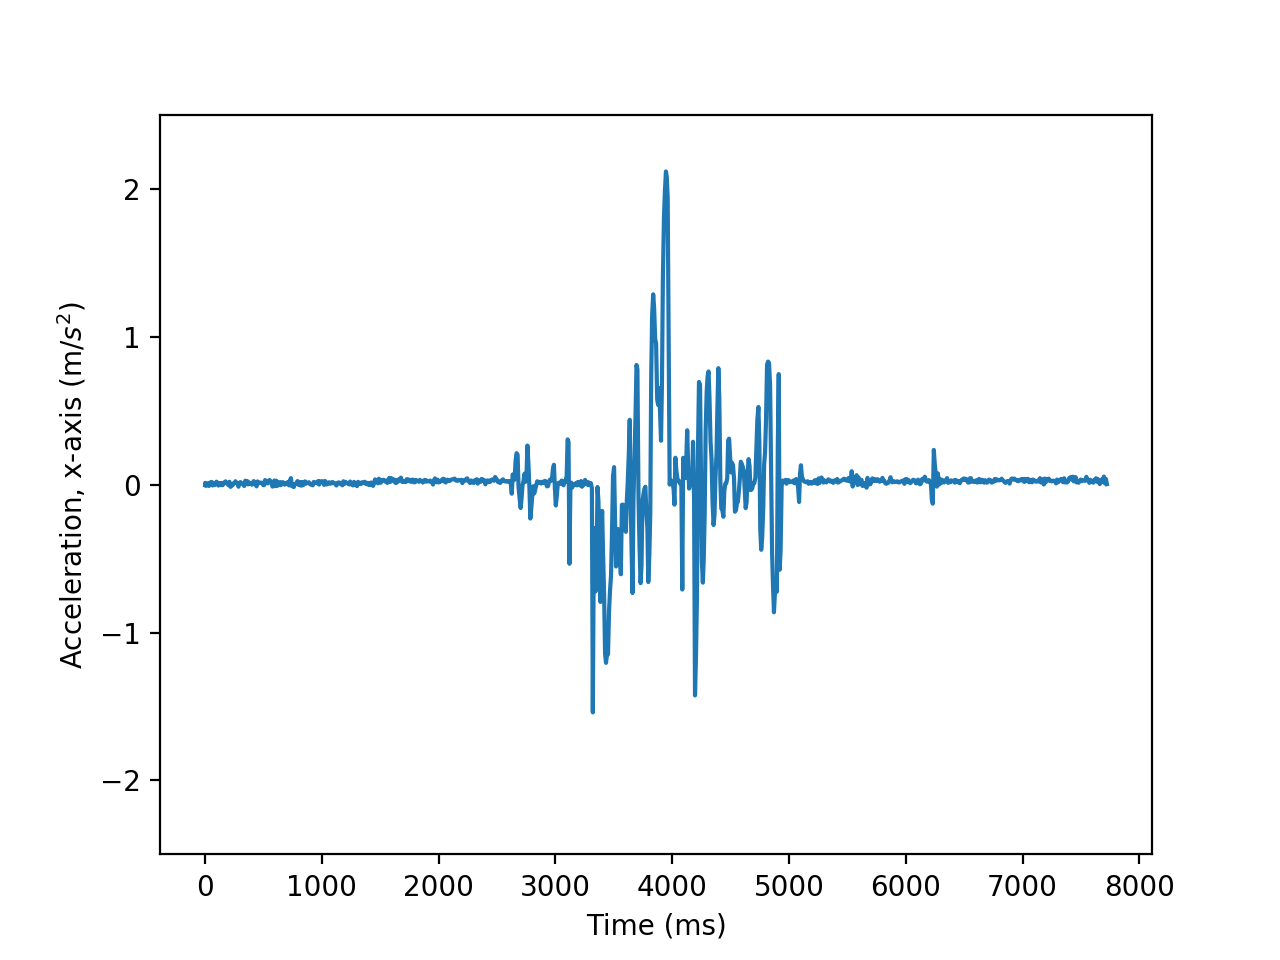
\includegraphics[width=\linewidth]{f0-acc.png}
\caption{Frame 1, accelerometer input.}
\end{subfigure}

\begin{subfigure}[b]{.45\linewidth}
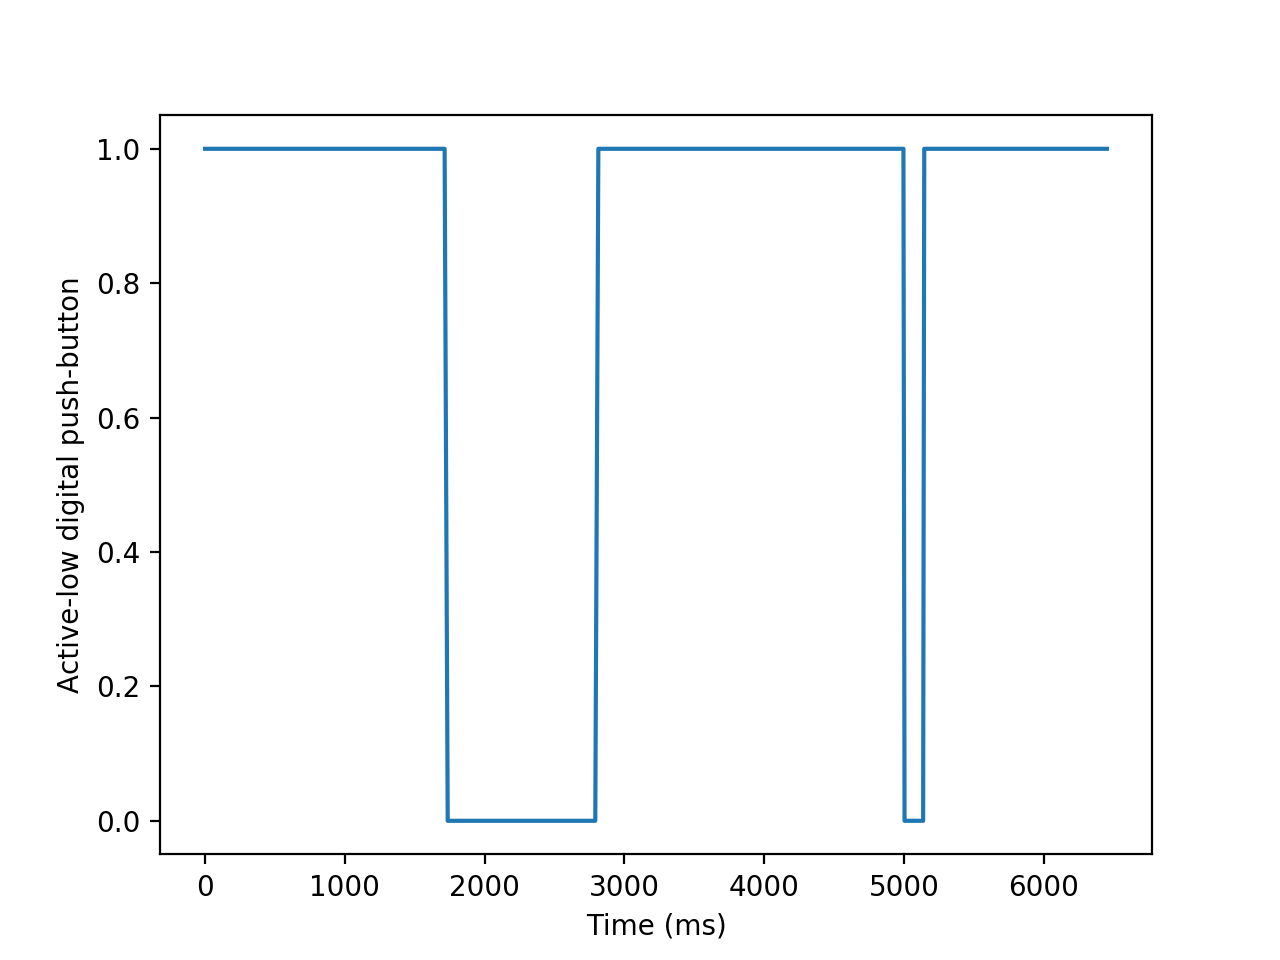
\includegraphics[width=\linewidth]{f1-button.png}
\caption{Frame 2, button input.}
\end{subfigure}
\begin{subfigure}[b]{.45\linewidth}
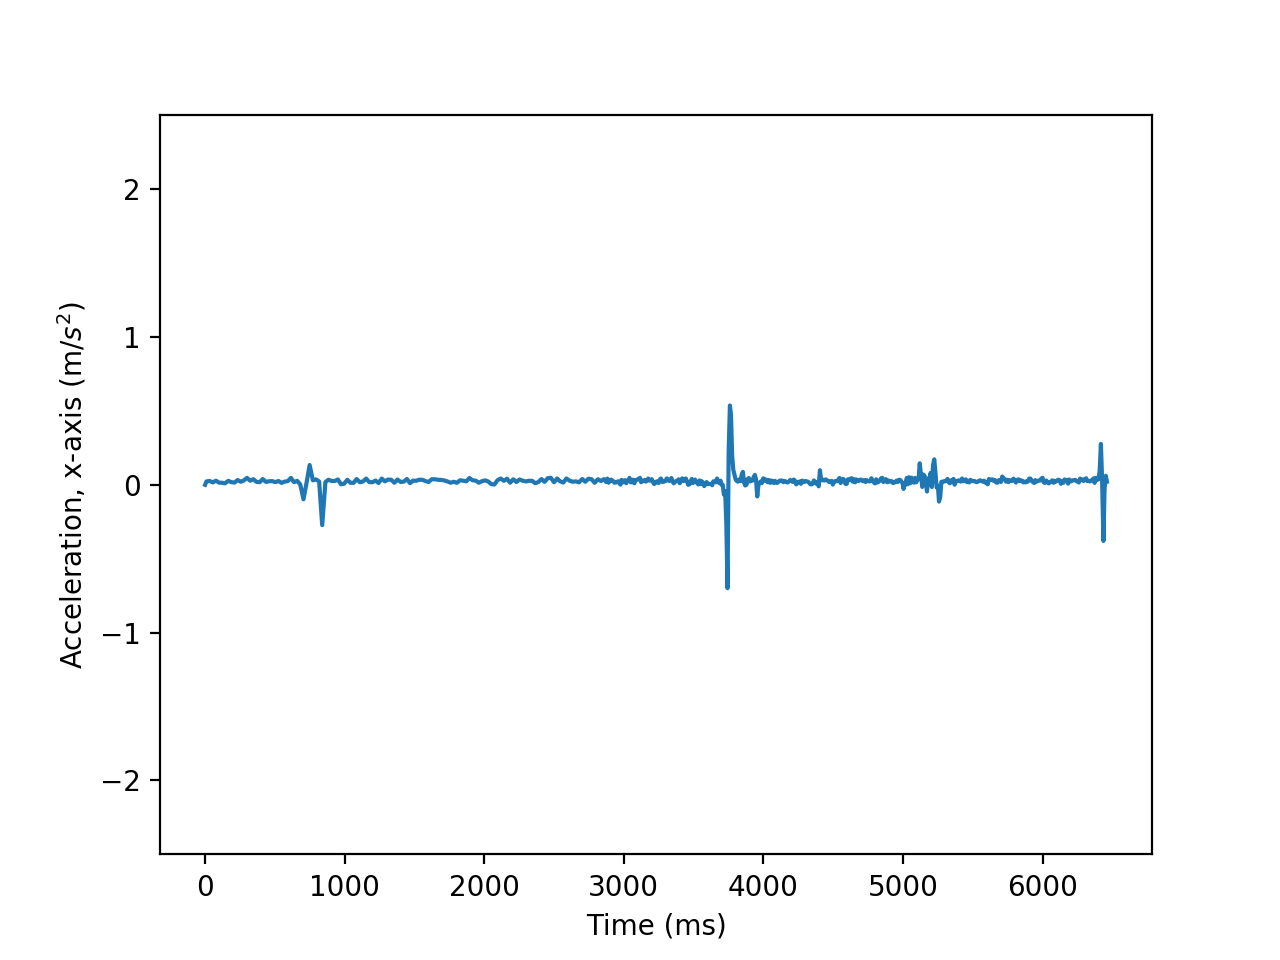
\includegraphics[width=\linewidth]{f1-acc.png}
\caption{Frame 2, accelerometer input.}
\end{subfigure}

\caption{Visualization of value generating functions for both frames in automatically generated Wikipedia Scroller test.}
\label{fig:actual-input-frames}
\end{figure}

The Wikipedia Scroller exercise involves a single output channel, represented as a 128x64, bit map.  For that channel, we made the following selections for the instructor-specified attributes: 0.8 for the required portion of each evaluation point, and ``text equality" for the check function.  The ``text equality" function checks if two bitmaps contain images of the same text.   Combining these preferences with the recording, MicroGrader constructed the evaluation points described in Table \ref{table:actual-points}.  For conciseness, the table refers to the start condition of frame 1 as $C_1$ and the start condition of Frame 2 as $C_2$.

\begin{table}
\begin{center}
\vspace{2mm}
\begin{tabular}{>{\centering\arraybackslash} m{3.75cm} >{\centering\arraybackslash} m{3cm} >{\centering\arraybackslash} m{1.5cm} >{\centering\arraybackslash} m{2.5cm} >{\centering\arraybackslash} m{1.5cm} }
Expected Value & Check Function & Condition & Interval & Portion \\ \hline \vspace{2mm}
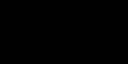
\includegraphics[width=\linewidth]{screen-blank.png} & Text equality & $C_1$ & (0,2581) & 0.8 \\
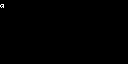
\includegraphics[width=\linewidth]{screen-a.png} & Text equality & $C_1$ & (2581,3177) & 0.8 \\ % a
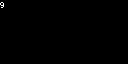
\includegraphics[width=\linewidth]{screen-9.png} & Text equality & $C_1$ & (3177,3744) & 0.8 \\ % 9
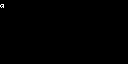
\includegraphics[width=\linewidth]{screen-a.png} & Text equality & $C_1$ & (3744,3895) & 0.8 \\ % a
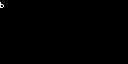
\includegraphics[width=\linewidth]{screen-b.png} & Text equality & $C_1$ & (3895,4046) & 0.8 \\ % b
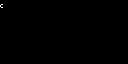
\includegraphics[width=\linewidth]{screen-c.png} & Text equality & $C_1$ & (4046,5690) & 0.8 \\ % c
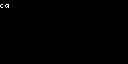
\includegraphics[width=\linewidth]{screen-ca.png} & Text equality & $C_1$ & (5690,7812) & 0.8 \\ % ca
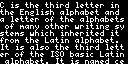
\includegraphics[width=\linewidth]{screen-wiki-c.png} & Text equality & $C_2$ & (0,2840) & 0.8 \\ % wiki "c"
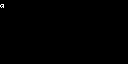
\includegraphics[width=\linewidth]{screen-a.png} & Text equality & $C_2$ & (2840,5183) & 0.8 \\ % a
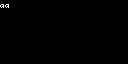
\includegraphics[width=\linewidth]{screen-aa.png} & Text equality & $C_2$ & (5183,6556) & 0.8 \\ \hline % aa
\end{tabular}
\caption{Automatically constructed evaluation points for Wikipedia Scroller.}
\label{table:actual-points}
\end{center}
\end{table}

In practice, this automatically constructed test was effective at grading this assignment.  We made a variety of minor changes to the reference implementation.  Some of these changes did not affect the system's adherence to the specification of the exercise, such as the exact positioning of text on the screen.  Using the generated test, MicroGrader correctly gave these implementations full credit.  Other changes resulted in a system that did not quite meet the specification, and MicroGrader correctly gave these less-than-perfect scores.

\clearpage
\section{Future Work}
MicroGrader can successfully execute tests on students' embedded systems.  It can also automatically generate tests using a recording of an instructor's system.  Nevertheless, the project is not finished; MicroGrader is being actively developed further.  In this section, we outline a few improvements that future versions will bring.

\subsection{Custom data types}
In the current implementation of MicroGrader, adding new data types for input and output channels requires modifying the source code.  In the next version, it will be possible to specify a custom data type in a separate Python file.  The file will include the name of the data type, as well as the implementations of certain necessary functions.  Namely, there must be functions to serialize and deserialize the data type, and the equality operator must be implemented.

\subsection{Additional timing flexibility}
It is currently difficult for instructors to have loose specifications with regards to time shifts, since evaluation points have fixed intervals relative to a condition.  The only flexibility is picking a condition to which that interval is relative.  In the next version of MicroGrader, the data structure for test cases will be augmented such that an instructor can give different sorts of timing specification.  For example, an instructor could specify that a certain sequence of output values must occur in a certain order, regardless of timing.  It will also be possible to put requirements on the length of time for which an output value occurs, regardless of exactly when it occurs.

\subsection{Editing automatically generated test cases}
A significant problem with automatically generated test cases is that of ambiguity.  The test case might prescribe inputs that can have multiple reasonable outputs.  For example, a test case for Wikipedia Scroller might involve a ``tilt" input in query-entry mode that should cause the selected character to scroll $n$ indices forward, but is very close to causing the character to scroll $n+1$ indices forward.  Instructors may not want to penalize students whose systems scroll one character too far, but the automatically generated test case will penalize these students.  Instructors, therefore, might want to edit the test case to disambiguate the tilt input so that its duration is further from an edge case.  A future version of MicroGrader will include tools for making changes to existing test cases.

\subsection{Dynamic values}
Certain ``correct" values are not determined at the time the test case is created.  For example, the Wikipedia Scroller assignment has an output that involves the current text on Wikipedia.org.  The next version of MicroGrader, will include a ``place-holder" data type.  This placeholder will be a function that runs at evaluation time to generate the correct value.  In the Wikipedia Scroller case, the placeholder would fetch the correct text from Wikipedia.

\subsection{Second order outputs}
As mentioned in section \ref{sec:derived-outputs}, it is sometimes desirable to measure an output that is not directly generated by the microcontroller, but rather is some transformation of an output generated by the microcontroller.  In the next version of MicroGrader, instructors will have the ability to specify a transformation to convert the microcontroller's outputs to a derived output (e.g. converting a motor voltage to the position of an attached wheel).

\clearpage
\begin{appendices}
\section{Client-server protocol}
\label{sec:protocol}
All client-server communication occurs over a USB connection.  All multi-byte integers are transmitted in a little-endian fashion.  In general, we refer to a message from the client to the server as a \textit{message}.  Some requests result in a server-to-client \textit{response}.  We use the term \textit{packet} to refer to a message or a response.

All packets consist of a header and a body.  The header contains important information about the packet, and specifies the length of the body. Thus, our protocol requires no termination byte.  A packet is considered complete once the expected number of bytes is received.  As a result, all packet bodies must have the specified length, or further communication will fail.

The basic structure of a message is as follows:

\textbf{message ::= $<$message header$>$$<$message body$>$}

\textbf{message header ::= $<$uint8 code$>$$<$uint32 timestamp$>$$<$uint16 body length$>$}

\noindent The most significant bit of the message code byte determines whether or not the server should send a response.  If the bit is 0, a response should be sent.  If the bit is 1, a response should be omitted.  The lower seven bits of the code determine the type of message, and therefore, how the message body should be interpreted.  The structure of the message body depends on the particular type of message.  The timestamp is measured in milliseconds, and the body length is measured in bytes.

The basic structure of a response is as follows:

\textbf{response ::= $<$response header$>$$<$response body$>$}

\textbf{response header ::= $<$uint8 code$>$$<$uint16 body length$>$}

\noindent The second-least significant bit of the response code indicates whether or not an error occurred with the most recent request (1 indicates an error occurred, 0 indicates success).  The response body for an error response is always empty.

The least significant bit indicates if the current session is complete (1 indicates yes, 0 indicates no).  The server disconnects immediately after sending a response indicating the session is complete.  Once again, the body length is measured in bytes.  Notice that the server does not include a timestamp in the response header.  The structure of the response body depends on the type of message to which the response corresponds.

Broadly speaking, there are three kinds of messages: input messages, output messages, and event messages.

\subsection{Inputs}
Input messages are typically used to ``inject" pre-determined test values, in place of true sensor readings.  Alternatively, input messages can be used to record observed sensor values on an instructor's system, for the purpose of building tests.  Table \ref{table:input-messages} describes the message bodies for input messages.

\begin{table}[ht]
\begin{center}
\begin{tabular}{l l l}
code & name & message body \\ \hline
0x20 & Digital Input & $<$uint8 pin$>$[$<$uint8 value$>$] \\
0x22 & Analog Input & $<$uint8 pin$>$$<$analog params$>$[$<$int32 value$>$] \\
0x30 & Accelerometer & $<$analog params$>$[$<$int32 x value$>$$<$int32 y value$>$$<$int32 z value$>$] \\
0x31 & Gyroscope & $<$analog params$>$[$<$int32 x value$>$$<$int32 y value$>$$<$int32 z value$>$] \\
0x32 & Magnetometer & $<$analog params$>$[$<$int32 x value$>$$<$int32 y value$>$$<$int32 z value$>$] \\ \hline
\end{tabular}
\caption{Summary of contents of input messages.}
\label{table:input-messages}
\end{center}
\end{table}

If the optional value or values are included, this message is reporting recorded sensor readings from the client to the server.  In that case, the body of the response (if there is a response) is empty.  

If the optional values are not included, this message is requesting test values.  In that case, the body of the response (if there is a response), is just the requested values.  For digital input requests, the response is a single byte containing a 0 or a 1.  For analog input requests, the response is a 32-bit integer.  For the accelerometer, gyroscope, and magnetometer requests, the response is a sequence of three 32-bit bit integers representing the x-value, y-value, and z-value respectively.

\subsubsection{Value Encoding}
Encoding for digital values is simple: a single byte containing the value 0 or 1.  For analog values, however, MicroGrader uses a system by which the client decides how an analog value becomes discretized.  In particular, the client specifies the \textit{analog params} which are defined as follows:

\footnotesize
\textbf{analog params ::= $<$int32 min bin$>$$<$int32 max bin$>$$<$int32 min value$>$$<$int32 max value$>$}
\normalsize

\noindent These parameters indicate that the physical quantity in the range (min value, max value) should be mapped to the range (min bin, max bin) for discretization.

To illustrate, we examine the behavior of the Teensy client for analog input requests.  It uses the values 0 and 3300 for \texttt{min value} and \texttt{max value} respectively.  These represent the minimum and maximum voltages, in millivolts, that the Teensy's analog-to-digital converter (ADC) can process.  For \texttt{min bin} and \texttt{max bin}, the values depend on the Teensy's current analog resolution.  If the resolution is 10 bits for example, the Teensy client would use the values 0 and 1023 for \texttt{min bin} and \texttt{max bin}.

Suppose the Teensy makes a request for an analog input using these parameters, and the server observes that the true value to ``inject" is $x$.  Let $b_{\text{min}}$, $b_{\text{max}}$, $v_{\text{min}}$, and $v_{\text{max}}$ represent the min bin, max bin, min value, and max value respectively.  The server must convert the value $x$ to a ``bin number", $y$, in accordance with the given parameters:

$$y = \left \lfloor b_{\text{min}} + \frac{x_{\text{bound}}-v_{\text{min}}}{v_{\text{max}}-v_{\text{min}}} * (b_{\text{max}}-b_{\text{min}}) \right \rfloor$$

where

$$x_{\text{bound}} = \min(v_{\text{max}}, \max(v_{\text{min}}, x))$$

The server responds with the value $y$.  Now consider a situation in which the client reports an input sample to the server, rather than requesting an input value.  For such input ``recordings", the value supplied by the client should also be the bin number as described by the above formula (typically this math would be calculated in hardware by the ADC).

\subsubsection{Units}
The units for analog requests are not specified.  There is no built-in unit for the relevant physical quantities (namely voltage, acceleration, angular velocity, and magnetic flux density).  The client implementation and the constructed test cases just need to be consistent.  For example, the reference Teensy client implementation uses millivolts for voltage, and any test cases written for this client should use values expressed in millivolts.

\subsection{Outputs}
Output messages are used to report outputs to the server.  Table \ref{table:output-messages} describes the message bodies for output messages.

\begin{table}[ht]
\begin{center}
\begin{tabular}{l l l}
code & name & message body \\ \hline
0x21 & Digital Output & $<$uint8 pin$>$$<$uint8 value$>$ \\
0x23 & Analog Output & $<$uint8 pin$>$$<$analog params$>$$<$int32 value$>$ \\
0x41 & Screen & $<$tile$>$* \\
\end{tabular}
\caption{Summary of contents of output messages.}
\label{table:output-messages}
\end{center}
\end{table}

If the client specifies that a response should be sent, then the body of the response is empty.  The encoding of values for digital outputs is the same as for digital inputs (a single byte, 0 or 1).  The encoding of values for analog outputs is the same as for analog inputs.  Recall that the value reported is a ``bin number".

\subsubsection{Screen Encoding}
Since the built-in screen type is a monochrome display, in which each pixel is on-or-off, our screen is essentially a bitmap.  We represent each pixel using a single bit.  Our encoding for the screen is inspired by the U8x8 embedded library \cite{u8x8}, and it makes it simple for embedded clients to transmit screen information if their display libraries are U8x8 compatible.

We encode the screen as a collection of 8x8 \textit{tiles}.  The entire bitmap for a tile is contained in an unsigned 64-bit integer.  The most significant byte of the 64-bit integer encodes the leftmost column of the tile.  The next-most significant byte encodes the second-to-leftmost column of the tile, and so forth.  Within a 8-pixel column, the most significant bit represents the state (on or off) of the top pixel, the second-most significant bit represents the state of the pixel below that, and so forth.  In our terminology, the leftmost column has the coordinate $x=0$ and the topmost row has the coordinate $y=0$.  Therefore, the point $(0, 0)$ is the top-left corner of a bitmap.  When a tile is transmitted over serial, note that this unsigned 64-bit integer, like all our other multi-byte integers, are transmitted in a little-endian fashion.  So the lowest-order byte, representing the rightmost column of the tile, is transmitted first.

The screen can be considered a grid of non-overlapping tiles (though padding might be necessary so that 8x8 tiles perfectly cover the entire screen.  When transmitting the screen, the tiles are transmitted by row, from top to bottom (lowest y-coordinate to highest y-coordinate.  Within each row, tiles are transmitted from right to left (highest x-coordinate to lowest x-coordinate).  Note that the Screen request does not specify the shape of the screen; it just sends a sequence of tiles.  Therefore, it is imperative that, before sending any Screen requests, the client informs the server of the screen shape using a ``Screen Init" request (see section \ref{sec:event-messages}).

\subsection{Events}
\label{sec:event-messages}
Event messages are similar to output messages in that they are used to report information to the server, not receive information from the server.  Responses to event messages have empty bodies, just as with output messages.  Table \ref{table:event-messages} describes the bodies of event messages.

\begin{table}[ht]
\begin{center}
\begin{tabular}{l l l}
code & name & request body \\ \hline
0x00 & Init & (\textit{empty}) \\
0x01 & Print & $<$uint8 char$>$* \\
0x40 & Screen init & $<$uint8 width$>$$<$uint8 height$>$ \\
0x50 & GPS fix & (\textit{empty}) \\
0x60 & HTTP request & (\textit{empty}) \\
0x61 & HTTP response & (\textit{empty}) \\ \hline
\end{tabular}
\caption{Summary of contents of event messages.}
\label{table:event-messages}
\end{center}
\end{table}

The ``Init" message is sent when the embedded client initializes.  In addition, the ``Screen Init" message is used upon initialization to inform the server of the width and height of the screen, as measured in 8x8 tiles.  The ``Print" message is used to send custom text (ASCII-encoded) from the client to the server.  This is particularly helpful for debugging, since it is impossible to perform regular debugging via USB when MicroGrader is in use.

It is important to inform the server of certain events, especially ones that have highly variable latencies.  The ``GPS Fix" message is used to inform the server that the client has acquired a GPS fix.  The ``HTTP request" message is used to inform the server that an HTTP request has been sent.  The ``HTTP response" message is used to inform the server that a internet response has been received.

\clearpage
\section{Client implementation for Teensy}
\label{sec:teensy}
MicroGrader is built to be cross-platform and is should work with a wide variety of microcontrollers.  As of now, the client side of the communication protocol is implemented for only one microcontroller development board: the Teensy.  The key for any client implementation is to be as invisible to students as possible.  In the case of the Teensy implementation, students implement projects in a \texttt{.ino} file, which has access to built-in functions.  In order to properly implement the protocol, I wrote a library that overrides many of these built-in functions to perform the proper communication with the server.  The required changes to the student's \texttt{.ino} file are minimal.

At its core, the client consists of a communication library that interacts with the server.  It provides functionality for other libraries to send messages to the server; the core communication library adds the message header to the message.  If the message requires a response, the communication library waits, and processes, that response, and returns its contents.  If the message does not require a response, the communication library returns immediately after sending a message.

The Teensy includes built-in functions to send and receive data over USB.  The MicroGrader client for Teensy replaces the built-in \texttt{Serial} object with a wrapper object.  When testing or recording, any print statements made using the \texttt{Serial} object have no effect.  For cases where a student or instructor wishes to print some text for debugging, the library includes a \texttt{debug} function, which sends a Print message in accordance with the MicroGrader protocol.  

The built-in functions for general purpose input-output functionality (GPIO) is also wrapped.  This allows for recording GPIO events and for injecting test inputs from the MicroGrader server.  For input from the inertial measurement unit (IMU), we modified the MPU9250 \cite{MPU9250} library for Arduino/Teensy.  For output to a display, we modified the U8g2 \cite{u8g2} library for Arduino/Teensy.  If an academic course uses the Teensy, but uses different libraries for IMU input and screen output, the course staff must modify the source code of those libraries.  Specifically, those libraries need to request inputs from the MicroGrader server when appropriate, instead of performing real sensor readings, and need to report information to the MicroGrader server when appropriate.  In practice, the code for doing this, with the help of the core communication library, is relatively simple.

The MicroGrader client for Teensy includes an \textit{inactive mode}, in which all built-in GPIO functions and third-party libraries operate normally, and in which there is no communication with the MicroGrader server.  In this mode, \texttt{Serial} print statements work normally.  Therefore, students can use \texttt{Serial} print statements when not connected to the MicroGrader server, but they do not have to worry about those statements interfering with MicroGrader communication when actual testing is happening.

From a student's perspective, very few changes need to be made in order to run the MicroGrader client.  He or she needs to install the core library and the modified versions of the third-party libraries.  The line \verb+#include "MicroGrader.h"+ must be added to the top of the \texttt{.ino} file and an initialization function, \texttt{MicroGrader.begin()} must be called at the beginning of the Teensy \texttt{setup()} routine.

\end{appendices}

\clearpage
\raggedright
\begin{thebibliography}{}
\bibitem{ut-austin-edx}
``Embedded Systems - Shape the World: Microcontroller Input/Output." \textit{EdX.}  Available at: 
https://www.edx.org/course/embedded-systems-shape-world-utaustinx-ut-6-10x.  Accessed September 1, 2017.

\bibitem{keil}
``MDK Microcontroller Development Kit." \textit{keil.com.}  Available at:
http://www2.keil.com/mdk5/. Accessed September 1, 2017.

\bibitem{catsoop}
``CAT-SOOP is an Automatic Tutor for Six-Oh-One Problems."  \textit{mit.edu.}  Available at:
https://catsoop.mit.edu/.  Accessed September 1, 2017.

\bibitem{wiki-scroller}
``Exercises 04."  \textit{mit.edu.} Available at:
https://iesc-s2.mit.edu/6S08/S17/EX04.  Accessed September 1, 2017.

\bibitem{teensy}
``Teensy USB Development Board."  \textit{PJRC} Available at:
https://www.pjrc.com/teensy/index.html.  Accessed September 1, 2017.

\bibitem{arduino-ide}
``Arduino IDE." \textit{Arduino.}  Available at:
https://www.arduino.cc/en/Main/Software.  Accessed September 1, 2017.

\bibitem{arduino-popular}
Torrone, Phillip.  "Why the Arduino Won and Why It?s Here to Stay."  \textit{Makezine.} Available at:
http://makezine.com/2011/02/10/why-the-arduino-won-and-why-its-here-to-stay/.  Accessed September 1, 2017.

\bibitem{arduino-students}
Hertzog, Pierre \& Swart, Arthur James. (2016). Arduino -- Enabling engineering students to obtain academic success in a design-based module. 10.1109/EDUCON.2016.7474533.

\bibitem{teensy-specs}
``Teensy 3.2 \& 3.1 -- New Features." \textit{PJRC.}  Available at:
https://www.pjrc.com/teensy/teensy31.html.  Accessed September 1, 2017.

\bibitem{MPU9250}
``SparkFun MPU-9250 Digital Motion Processor (DMP) Arduino Library." \textit{SparkFun.}  Available at: 
https://github.com/sparkfun/SparkFun\_MPU-9250-DMP\_Arduino\_Library.  Accessed September 1, 2017.

\bibitem{u8g2}
``U8g2."  \textit{GitHub.}  Available at: 
https://github.com/olikraus/u8g2/wiki.  Accessed September 1, 2017.

\bibitem{6s08-wifi}
``WiFi library for ESP8266." \textit{MIT 6.S08.}  Available at:
https://github.com/voldman/esp8266.  Accessed September 1, 2017.

\bibitem{python-popular}
Cass, Steven.  ``The 2017 Top Programming Languages" (2017).  \textit{IEEE}.  Available at: 
https://spectrum.ieee.org/computing/software/the-2017-top-programming-languages.  Accessed September 1, 2017.

\bibitem{python-ed}
Guo, Philip.  ``Python is Now the Most Popular Introductory Teaching Language at Top U.S. Universities" (2014).  \textit{ACM}.  Available at:
https://cacm.acm.org/blogs/blog-cacm/176450-python-is-now-the-most-popular-introductory-teaching-language-at-top-u-s-universities/fulltext.  Accessed September 1, 2017.

\bibitem{pyserial}
``Python serial port access library." \textit{GitHub.}  Available at:
https://github.com/pyserial/pyserial.  Accessed September 1, 2017.

\bibitem{tesseract}
``Tesseract Open Source OCR Engine." \textit{GitHub.} Available at:
https://github.com/tesseract-ocr/tesseract.  Accessed September 1, 2017.

\bibitem{5x7}
``fntgrpx11." \textit{GitHub.}  Available at:
https://github.com/olikraus/u8g2/wiki/fntgrpx11\#5x7.  Accessed September 1, 2017.

\bibitem{pickle}
``pickle -- Python object serialization." \textit{Python.org.}  Available at: 
https://docs.python.org/3/library/pickle.html.  Accessed September 1, 2017.

\bibitem{u8x8}
``U8x8." \textit{GitHub.}  Available at:
https://github.com/olikraus/u8g2/wiki/u8x8setupcpp.  Accessed September 1, 2017.

\end{thebibliography}
\end{document}